\chapter{Experimental results obtained}

\textcolor{green}{cateva sugestii:\\
1.	Trebuie facuta o scurta introducere care sa descrie pipeline-ul/flow-ul la tot ce ai facut. Cred ca o figura / o schema pt acest pipeline/flow ar ajuta mult sa se inteleaga cei 2 pasi: clasificare si localizare\\
2.	Descrierea datelor – ceea ce e acum in sect 4.1 si in sect 5.1\\
3.	Experimentele pentru clasificare\\
a.	Ceea ce e acum in sectiunea 5.2\\
b.	Eu as adauga la final o centralizare – un tabel cu 5 randuri (cele 5 experimente) in care as prezenta Acc, Precision(class_i), Recall(class_i), unde i=1,4 (la primele 3 modele) sau i=1,2 (la ultimele 2 modele)\\
4.	Experimente pentru detective \\
a.	Ceea ce e acum in sectiunea 5.3\\
b. 	Eu as adauga la final o centralizare intr-un tabel\\
5. Discutii si concluzii - care e cel mai ok clasific, resp detector pt a fi integrat in sistemul dezvoltat in capitolul urmator
}



\section{Data processing}

The process of defining and training both the classification model and the detection model started with gathering the data and learning how to work with dcm files because this was the first time I had an encounter with them. I quickly discovered that reading the images from the dcm files took a lot of time, which meant that training the models would also take a lot of time. These files contained the pixel data of about 50 slices, some had more and some had less, each representing images of width 2457 and height 1890, or 1996. I searched for ways to reduce the time for reading the files, at first by saving the slices as numpy arrays in file format, but that proved to not be ideal because it occupied a lot of disk storage. The dcm files themselves were not light either, totaling 120 GB of memory on my laptop, but the numpy arrays would have been impossible to store. Then, I arrived at the solution that, in time, proved to be the best: to save each individual slice as a png file. This meant that the time for reading the images was much faster, reading from dcm compared to png, and also that disk space was better utilized

In ~\cite{carte8} it is said that the input images for the object detection model should have a size divisible by 128, which I was not aware of when training the classification model, for which the images were not resized at all. I was training images of size 2457,1890 
\textcolor{green}{2457 $\times$ 1890?} 
\textcolor{green}{si ce ai facut cu cele care erau de dimensiunea 2457 $\times$ 1996?} 
on the GoogleNet model, but only taking a maximum of 5 slices from each image. After processing the dcm files, I found out that the lowest number of slices for an image in my entire subsection of the database was 22 therefore, for the purpose of properly balancing the database, I took into consideration only 22 slices of each image. 
\textcolor{green}{mai devreme ai zis ca imaginile contin 50 de slice-uri (eu am inteles ca fiecare contine 50; nu am inteles bine si unele au mai multe si unele au mai putine?)} 
For the images that had cancer, the ones that I had a file of bounding boxes on, I took the slice that had the tumor, 10 slices before that, and 11 after.

\section{Classification experiments}

I performed many experiments on the GoogleNet model for classification, and so I was able to understand how to work with 3D images. I first thought I had to stack them, so I sent the 5 slices that I selected from each image as 5 channels for the same input. That meant modifying the first convolutional layer of the GoogleNet architecture, which \textcolor{green}{originally} accepted inputs of 3$\times$W$\times$H 
\textcolor{green}{and now, in the current implementation, accepts inputs of 5$\times$W$\times$H}
. 
\textcolor{green}{eu as zice aici si de abordarea 2D si atunci acest paragraf e oarecum un preambul pt toate cele 5 experimente. Mai mult as avea grija ca la fiecare experiment sa precizezi f clar:\\
0. cate imagini in train, cate in test, cat de mari, cate clase sunt, cum sunt distribuite clasele in train si test\\
1. arhitectura clasificatorului (de ex la experimentul 1 e clar ca e arhitectura GoogleLeNet, dar la exp2 si exp3 nu e clar ce difera dpdv al arhitecturii (de ex. e bine sa spui ce are diferit aux1 de GoogleLeNet)\\
2. valorile (hyper)parametrilor folositi (optimiser, learning rate, policy of learning decay, loss fnction and the weights for it, batch size, number of steps/epochs)\\
3. evolutia loss-ului pe train (eventual si pe test)\\
4. performanta pe datele de test\\
Tu ai zis in text aceste lucruri, dar nu peste tot. De ex la exp4 si exp5, nu e clar care arhitectura se foloseste si care e distributia si nr datelor de train/test. Eu am lasat cu verde ce ar mai tb completat, dar te rog verifica si tu ca la fiecare experiemnt sa fie atinse cele 5 puncte de mai sus. Merci! :)
}


\subsection{Experiment 1}

The first experiment was made with a learning rate of 0.001, no learning rate decay, the optimizer was SGD, and the loss for every experiment, including this one, was cross-entropy. However, for the first few runs, I considered the problem of classification as a 4 label distinction, for which I attributed a different weight to the 4 labels: 1 for both normal and actionable, and 4 for benign and malign. 
\textcolor{green}{deci o problema de clasificare cu 4 clase (normal, actionable, beningn,malign), iar weight-urile folosite au fost: 1 pt normal, 1 pt actionable, 4 pt benign, 4 pt malign? Unde ai folosit weight-urile: in loss? daca da, cum le-ai integrat in CE?}
The batch size was 10
\textcolor{green}{eu stiu ca e bine sa fie putere de-a lui 2 sau multiplu de 8 parca la placile NVIDIA (probleme ce tin de performanta GPU-ului  cu procesoare virtuale si cele reale); matematic e corect cu orice valoare pt batch size, dar eu stiu aceasta valoare are impact asupra eficientei calculelor facute de GPU}
, and the images were not resized, so I was training images of width 2457 and height 1890. The batches were also not properly distributed, meaning that one single batch could have images of only one type. Each input consisted of 5 slices stacked on top of each other, representing 5 channels.
\textcolor{green}{deci nu ai folosit toate cele 22 de slice-uri, ci doar 5 (slice central +/- inca 2)?}
\textcolor{green}{e bine sa pui un tabel in care sa se vada cate imagini au fost in train, cate in validation/test, iar la train (si apoi la test) sa zici cate au fost normale, cate actionable, cate benign, cate malign} 

In order to track and compare each experiment, I used Weights \& Biases, also known as wanb, and logged the loss for each step, meaning that after each batch, the loss was calculated and added to the overall graph. Therefore, the image from Figure \ref{fig:fig8} shows the loss graph for the experiment described above.

\textcolor{green}{ai limitat si nr de epoci? Daca da, la cat? cati steps intra intr-o epoca? daca nu, ai limitat nr de steps? Daca da, la cat?}

\begin{figure}[!ht]
    \centering
    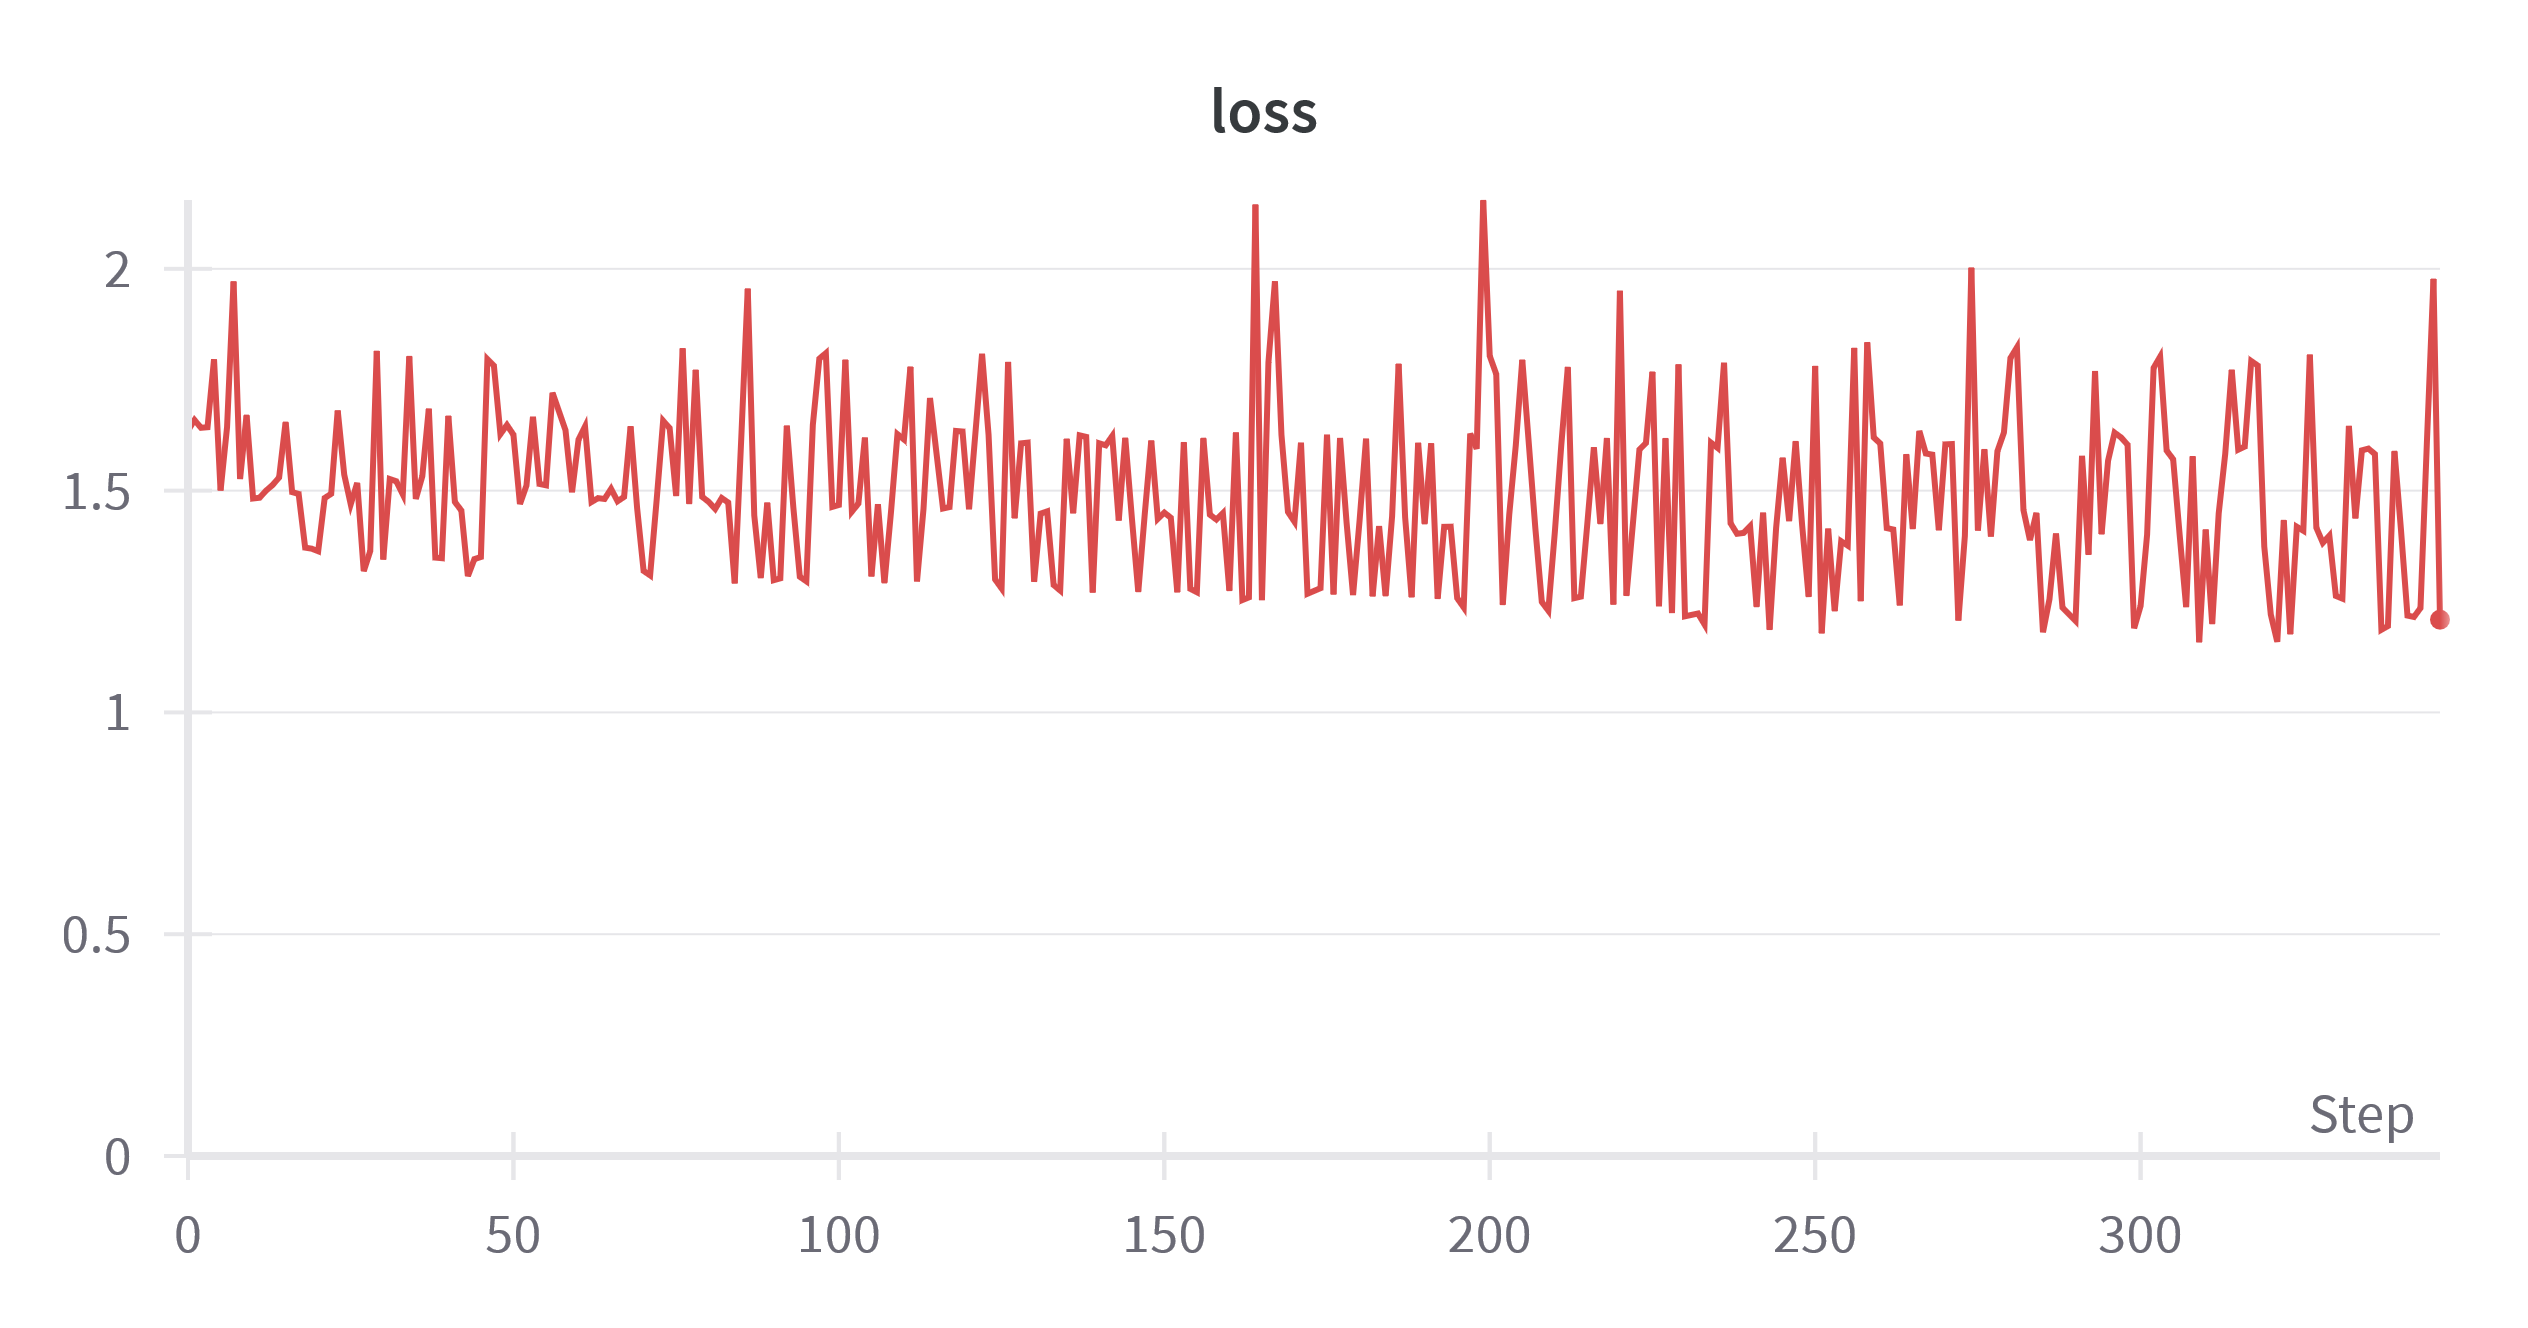
\includegraphics[width=1\textwidth]{figures/Figure8.png}
    \caption{Loss Graph
    \textcolor{green}{chiar daca ai zis deja in text, e bine sa rezumi in caption info despre: modelul folosit pt a obtine aceste rezultate si datele (train sau test) pt care s-a calculat aceasta performanta}
    }
    \label{fig:fig8}
\end{figure}

Evidently, the loss is not ideal. It does not appear to reduce its value after each step. This image (from Figure \ref{fig:fig8}) consists of the loss of the model calculated for 6 epochs 
\textcolor{green}{loss-ul din figura e pe setul de train?}
, and the predictions made on the test data was not ideal either, because it seemed to only predict normal or actionable types, disregarding the latter ones entirely. Figure \ref{fig:fig9} shows us how the confusion matrix looked after the first epochs, and after the sixth one.

\begin{figure}[!ht]
    \subfigure[]{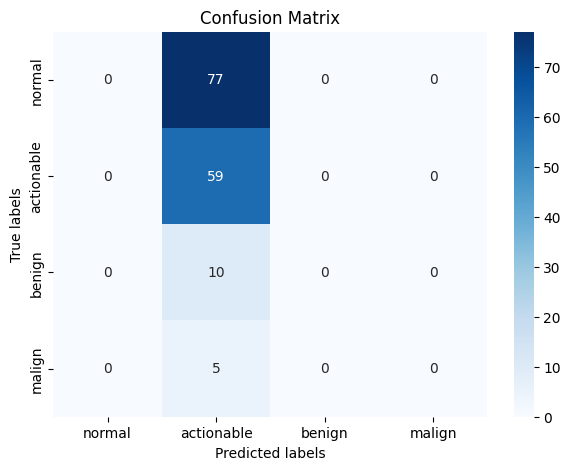
\includegraphics[width=0.45\linewidth]{figures/Figure9.png}}
    \subfigure[]{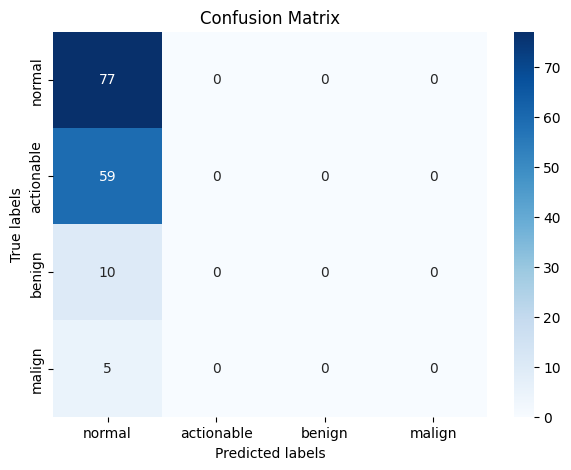
\includegraphics[width=0.45\linewidth]{figures/Figure10.png}}
    \caption{(a) After epoch 1 (b) After epoch 6
    \textcolor{green}{chiar daca ai zis deja in text, e bine sa rezumi in caption info despre: modelul folosit pt a obtine aceste rezultate si datele (train sau test) pt care s-a calculat aceasta performanta}
    }
    \label{fig:fig9}
\end{figure}

\subsection{Experiment 2}

The second experiment proved to be a little more fruitful. I changed the learning rate to 0.0001, the optimizer to Adam and employed learning rate decay, more exactly a step learning rate decay with a step size of 4 and a gamma of 0.1. The batch size was changed to 8 and I utilized a batch sampler class to correctly distribute the different input types into the batches in order to have a better proportion of classes. I was also under the impression that the GoogleNet architecture was maybe too deep to predict the images, so I experimented with the two auxiliary modules that GoogleNet provides. For this experiment, I trained the model using the first auxiliary while also modifying the forward-pass function to only include two inception layers.

\textcolor{green}{aici e nevoie sa dai mai multe detalii despre diferentele intre cele 2 arhitecturi incercate (sau sa faci un desen/o schita)}

Additionally, I changed the weights for the benign and malign classes in the loss function, substituting 4 for 6 for both of them. Figure \ref{fig:fig10} shows how the loss graph looked after training eight epochs and another 21 batches in the ninth epoch.

\begin{figure}[!ht]
    \centering
    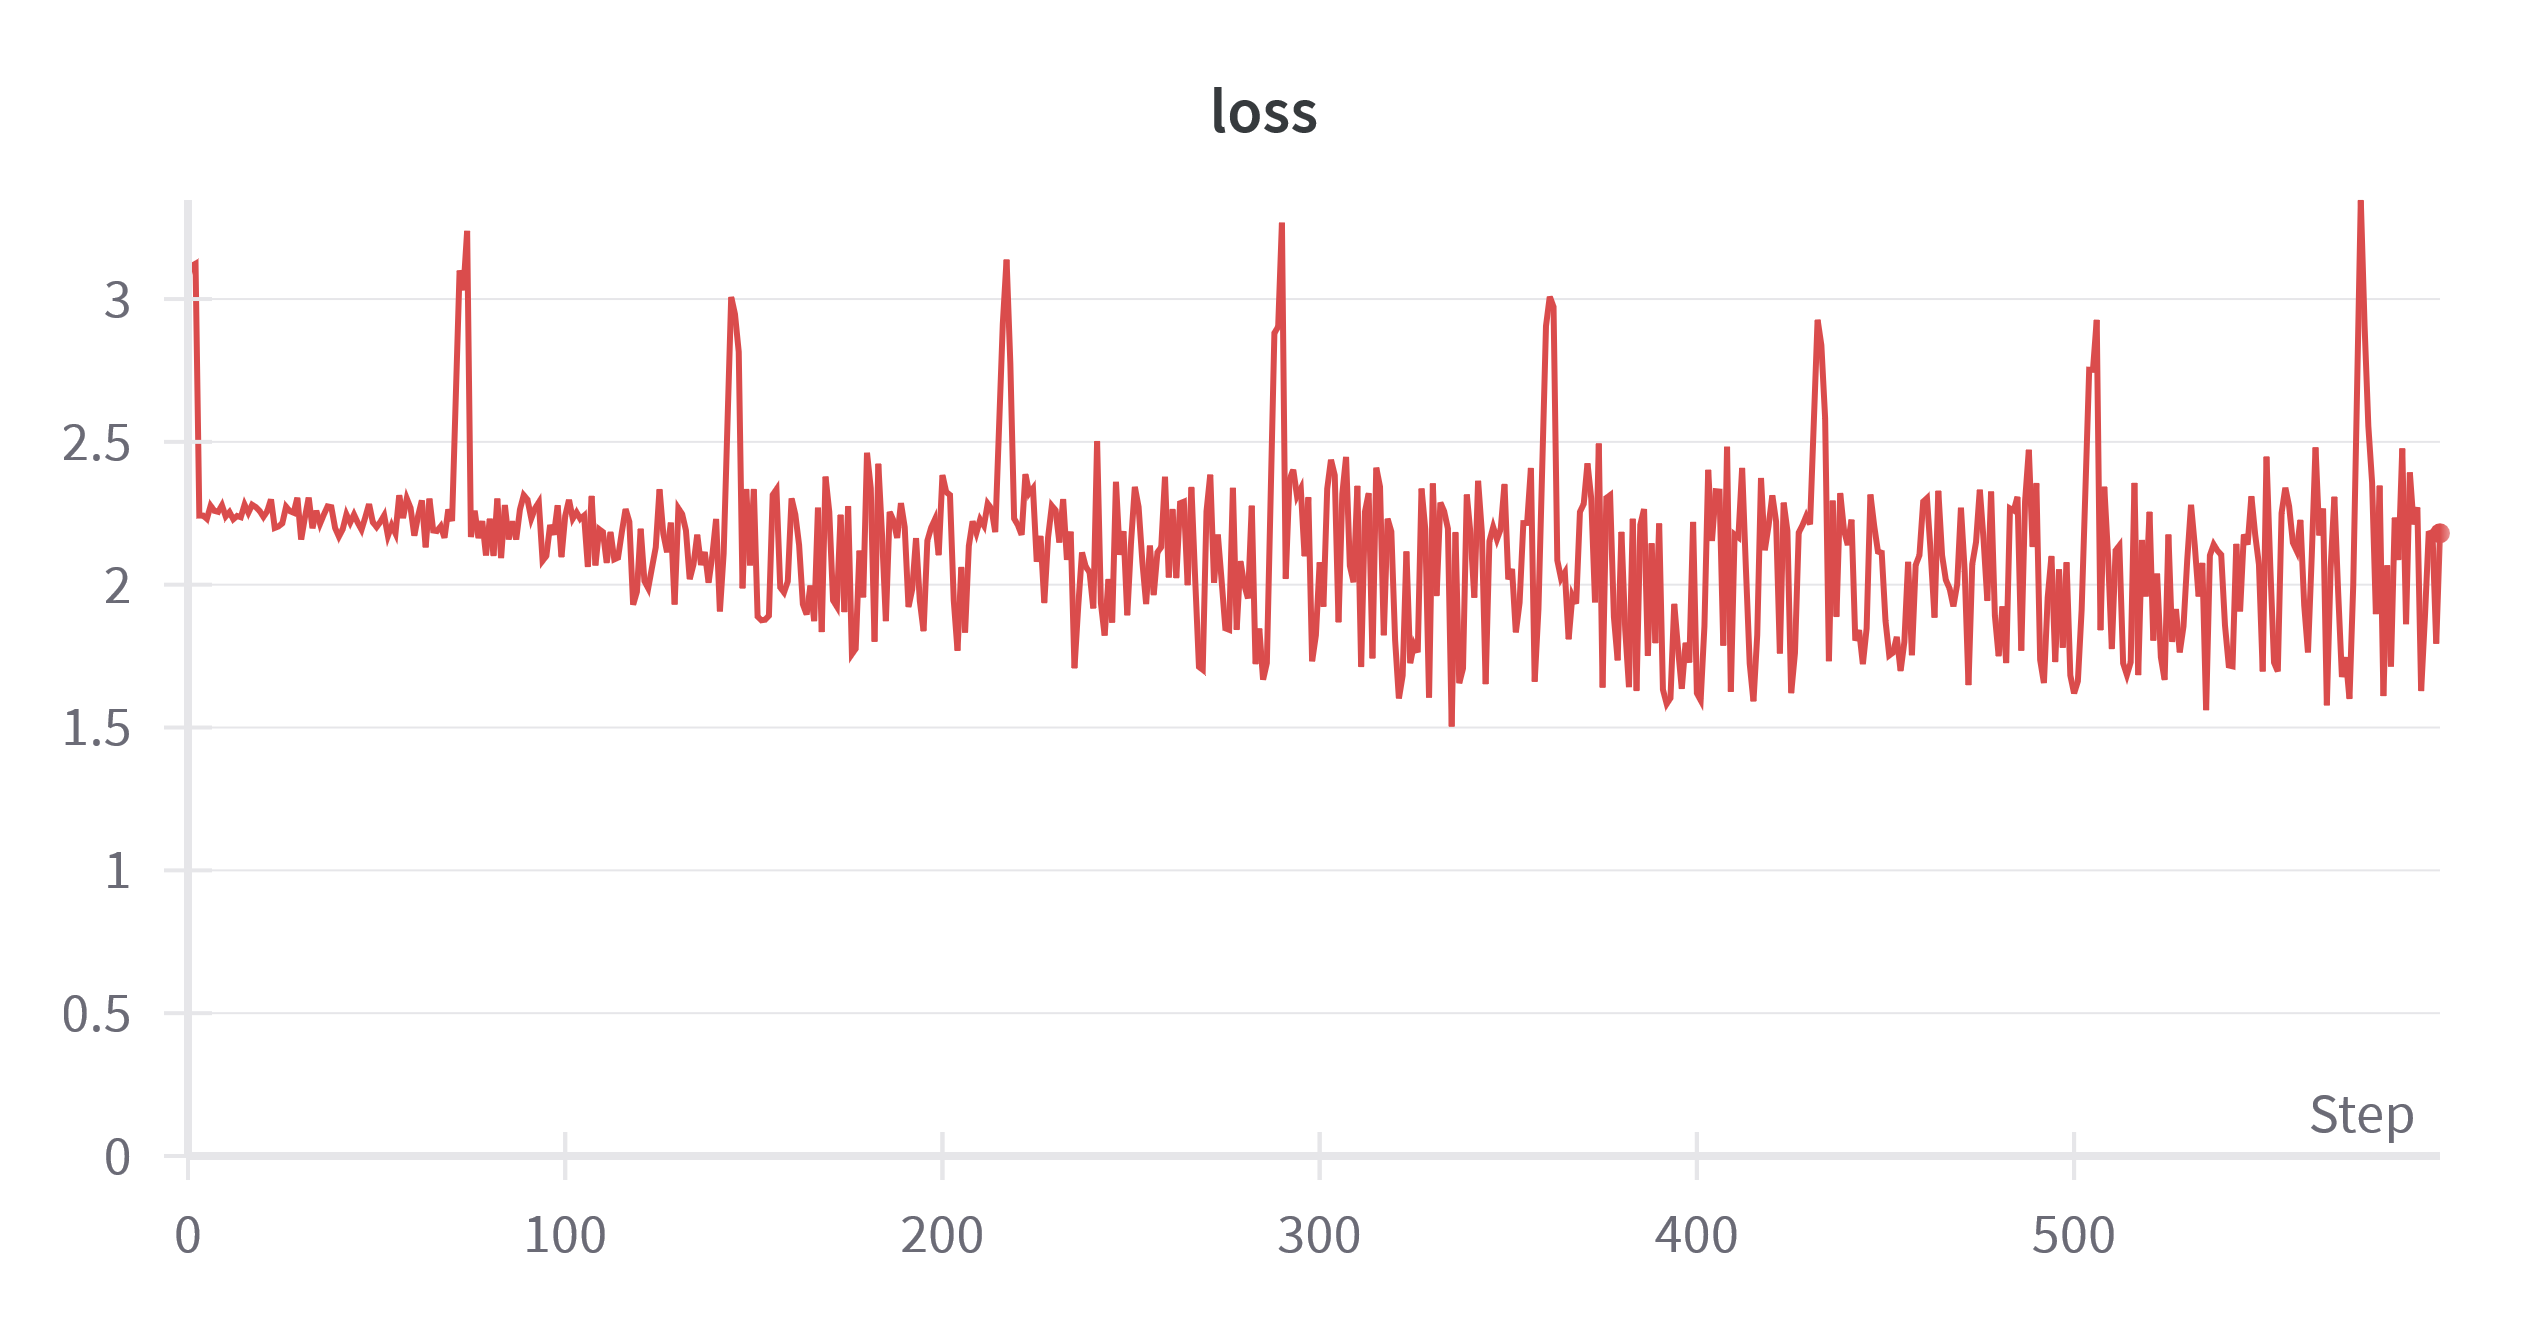
\includegraphics[width=1\textwidth]{figures/Figure11.png}
    \caption{Loss graph
    \textcolor{green}{chiar daca ai zis deja in text, e bine sa rezumi in caption info despre: modelul folosit pt a obtine aceste rezultate si datele (train sau test) pt care s-a calculat aceasta performanta} 
    }
    \label{fig:fig10}
\end{figure}

This time around, the model started to also predict images of class malign, but only after the first epoch. Curiously, it did not predict any images to be of type benign, even after eight epochs. Figure \ref{fig:fig11} shows how the predictions looked after the first and eighth epochs.

\begin{figure}[!ht]
    \subfigure[]{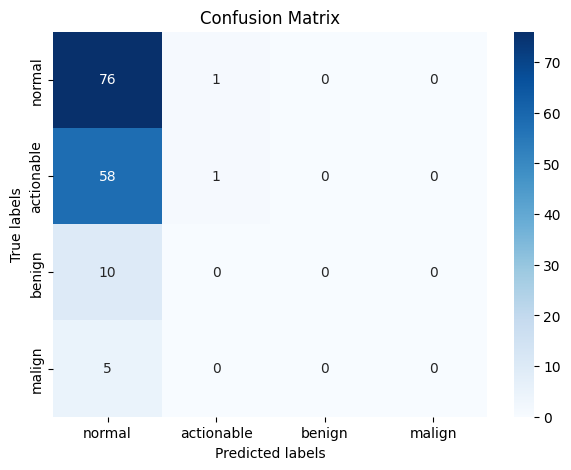
\includegraphics[width=0.45\linewidth]{figures/Figure12.png}}
    \subfigure[]{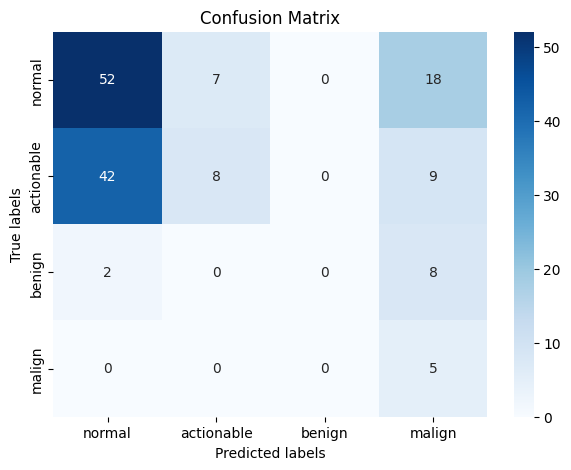
\includegraphics[width=0.45\linewidth]{figures/Figure13.png}}
    \caption{Classification performance (a) After epoch 1 (b) After epoch 8
    \textcolor{green}{chiar daca ai zis deja in text, e bine sa rezumi in caption info despre: modelul folosit pt a obtine aceste rezultate si datele (train sau test) pt care s-a calculat aceasta performanta}
    }
    \label{fig:fig11}
\end{figure}

\subsection{Experiment 3}

The only difference between this second experiment and the third was that the learning rate decay was changed from step to exponential with a gamma of 0.8. In Figure \ref{fig:fig13} is shown on the same graph the difference in loss between these two latter experiments.

\begin{figure}[!ht]
    \centering
    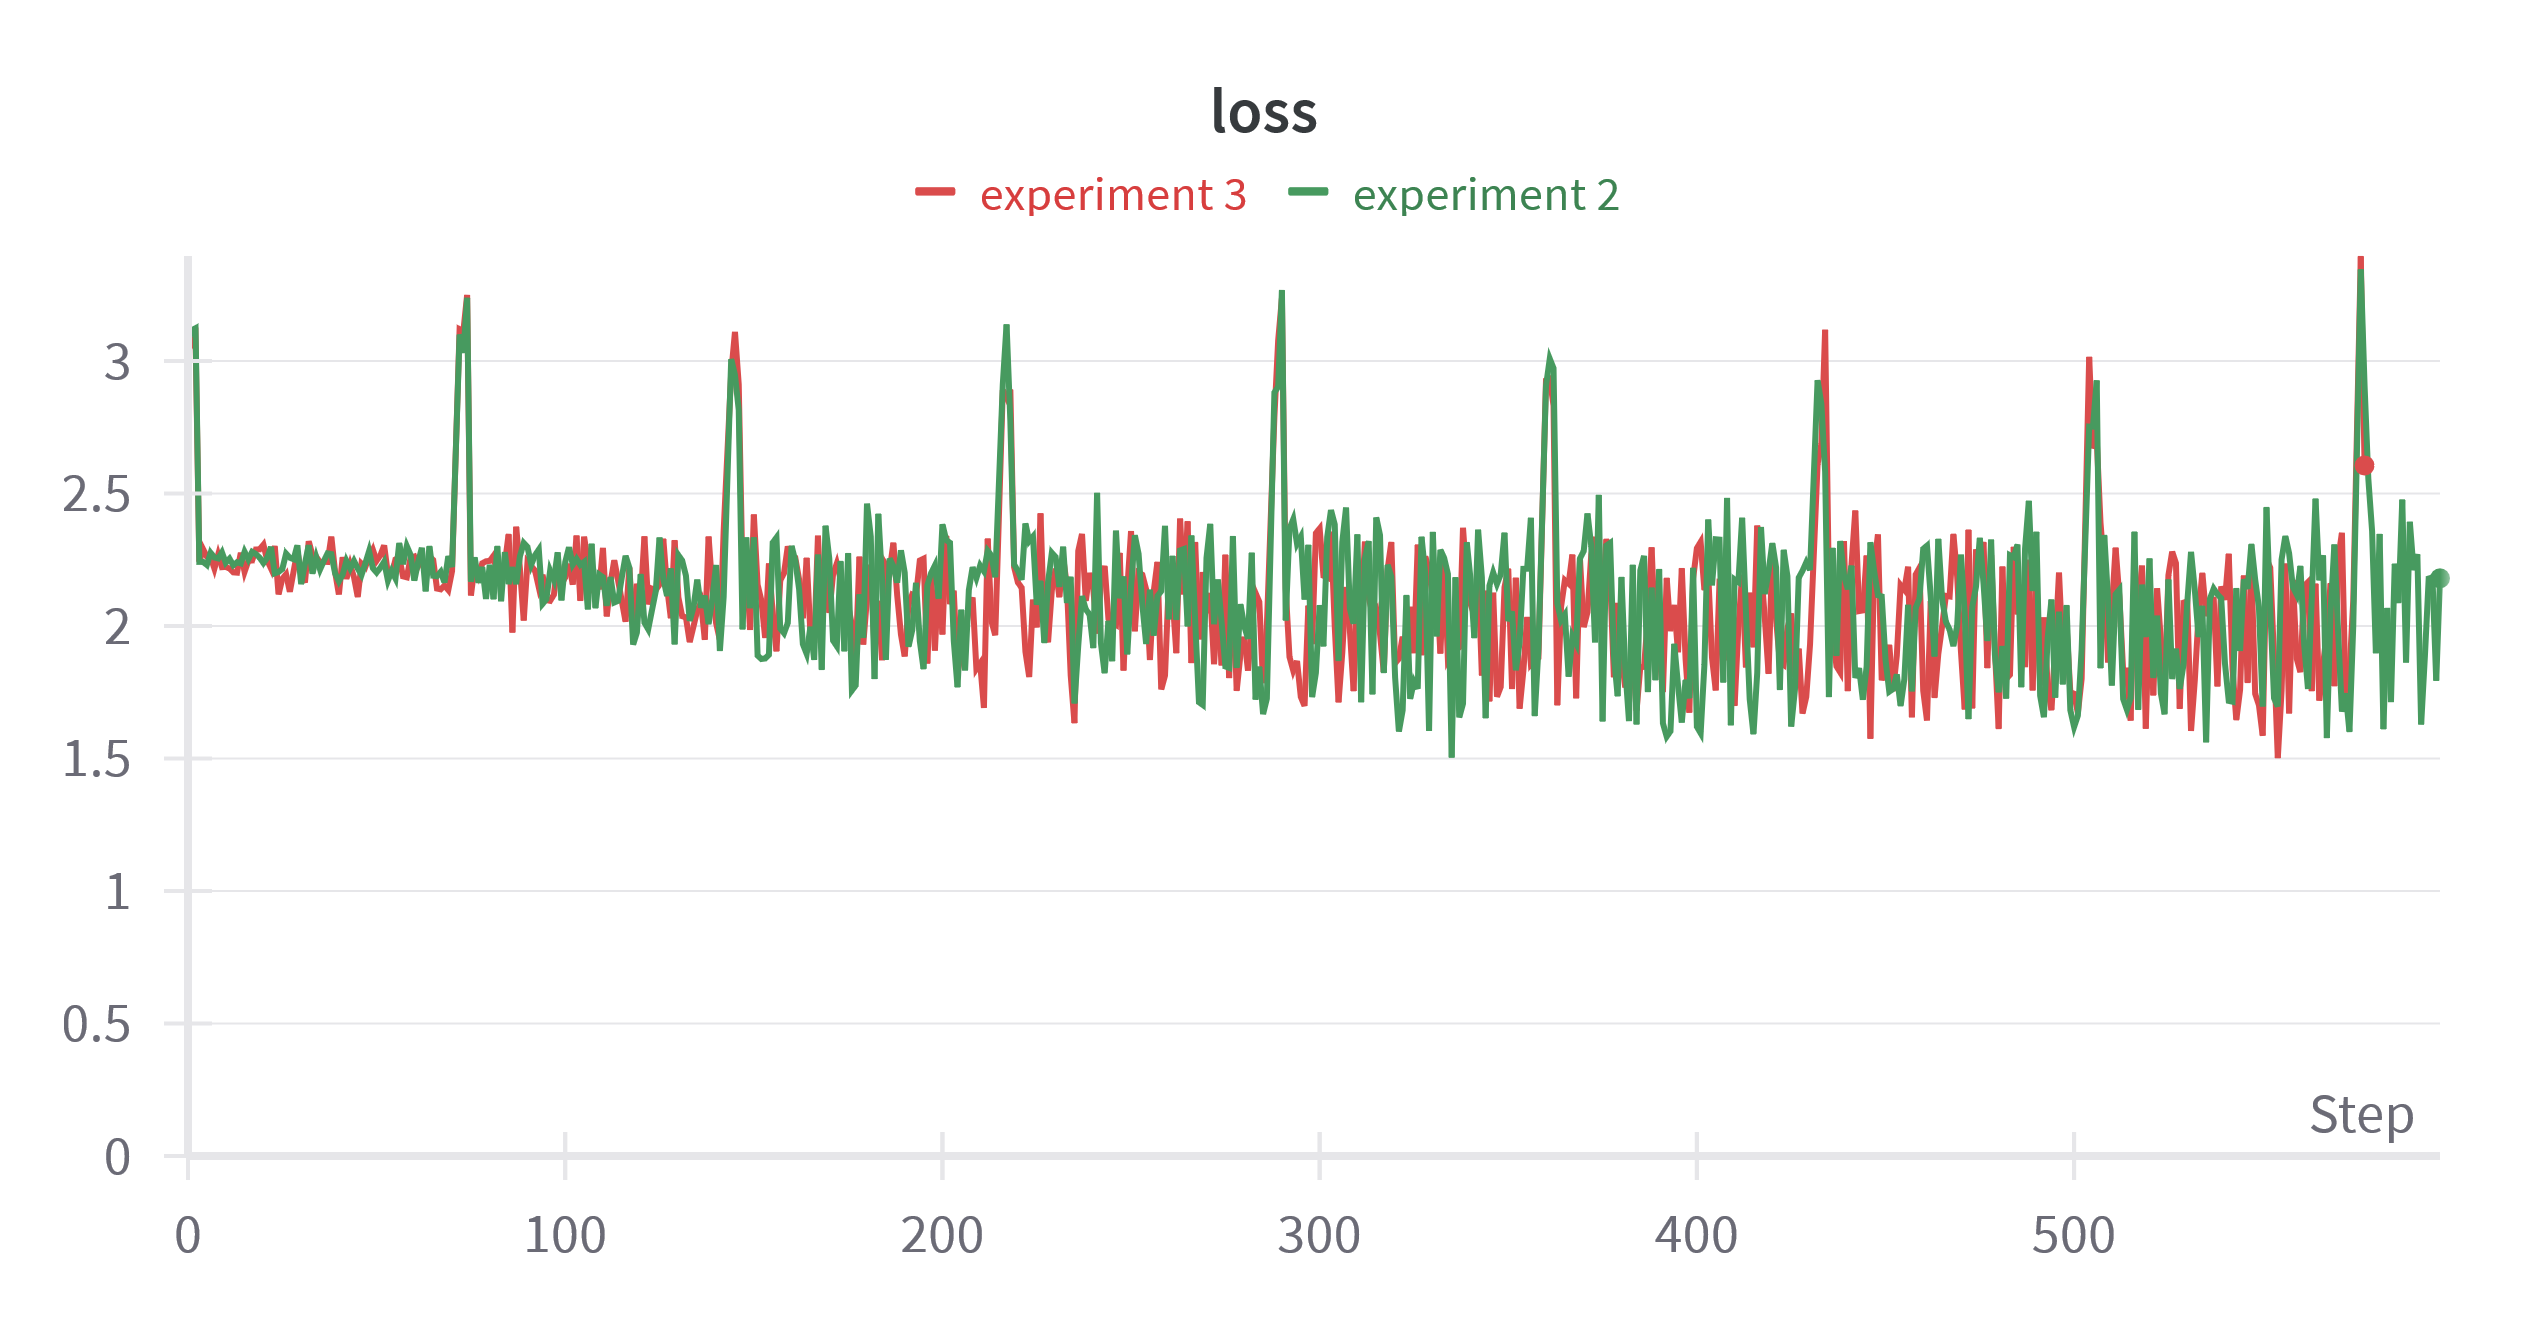
\includegraphics[width=1\textwidth]{figures/Figure14.png}
    \caption{Loss graph
    \textcolor{green}{chiar daca ai zis deja in text, e bine sa rezumi in caption info despre: modelul folosit pt a obtine aceste rezultate si datele (train sau test) pt care s-a calculat aceasta performanta}
    }
    \label{fig:fig13}
\end{figure}

The predictions for the third experiment were very similar to the ones from the second experiment, meaning the model would predict only three classes out of all four of them.

The spikes in Figure \ref{fig:fig10} represent the batches that had more input of classes benign and malign because the number of classes did not allow for equally proportionate batches of eight. I thought that the randomness in which these batches appeared could negatively impact the overall accuracy of the model, so in further experiments, I changed this way of thinking and made these batches appear first. Figure \ref{fig:fig13} shows how the experiment turned out, so not much was changed, and the predictions overall on the test data were not different.

\subsection{Experiment 4}

For the next experiment, I stopped considering this a problem of 4-label detection but rather a 2-label detection. Therefore, I grouped the actionable, benign and malign types into one and trained the model using this group and the normal ones. I kept everything else in terms of configuration from the third to the fourth experiment, except for batch size, which I changed to 64. Figure \ref{fig:fig16} shows how the loss looked after training three epochs
\textcolor{green}{on training data?} 
, and Figure \ref{fig:fig17} shows how the confusion matrix looked after those three epochs
\textcolor{green}{on testing data?}
.

\begin{figure}[!ht]
    \centering
    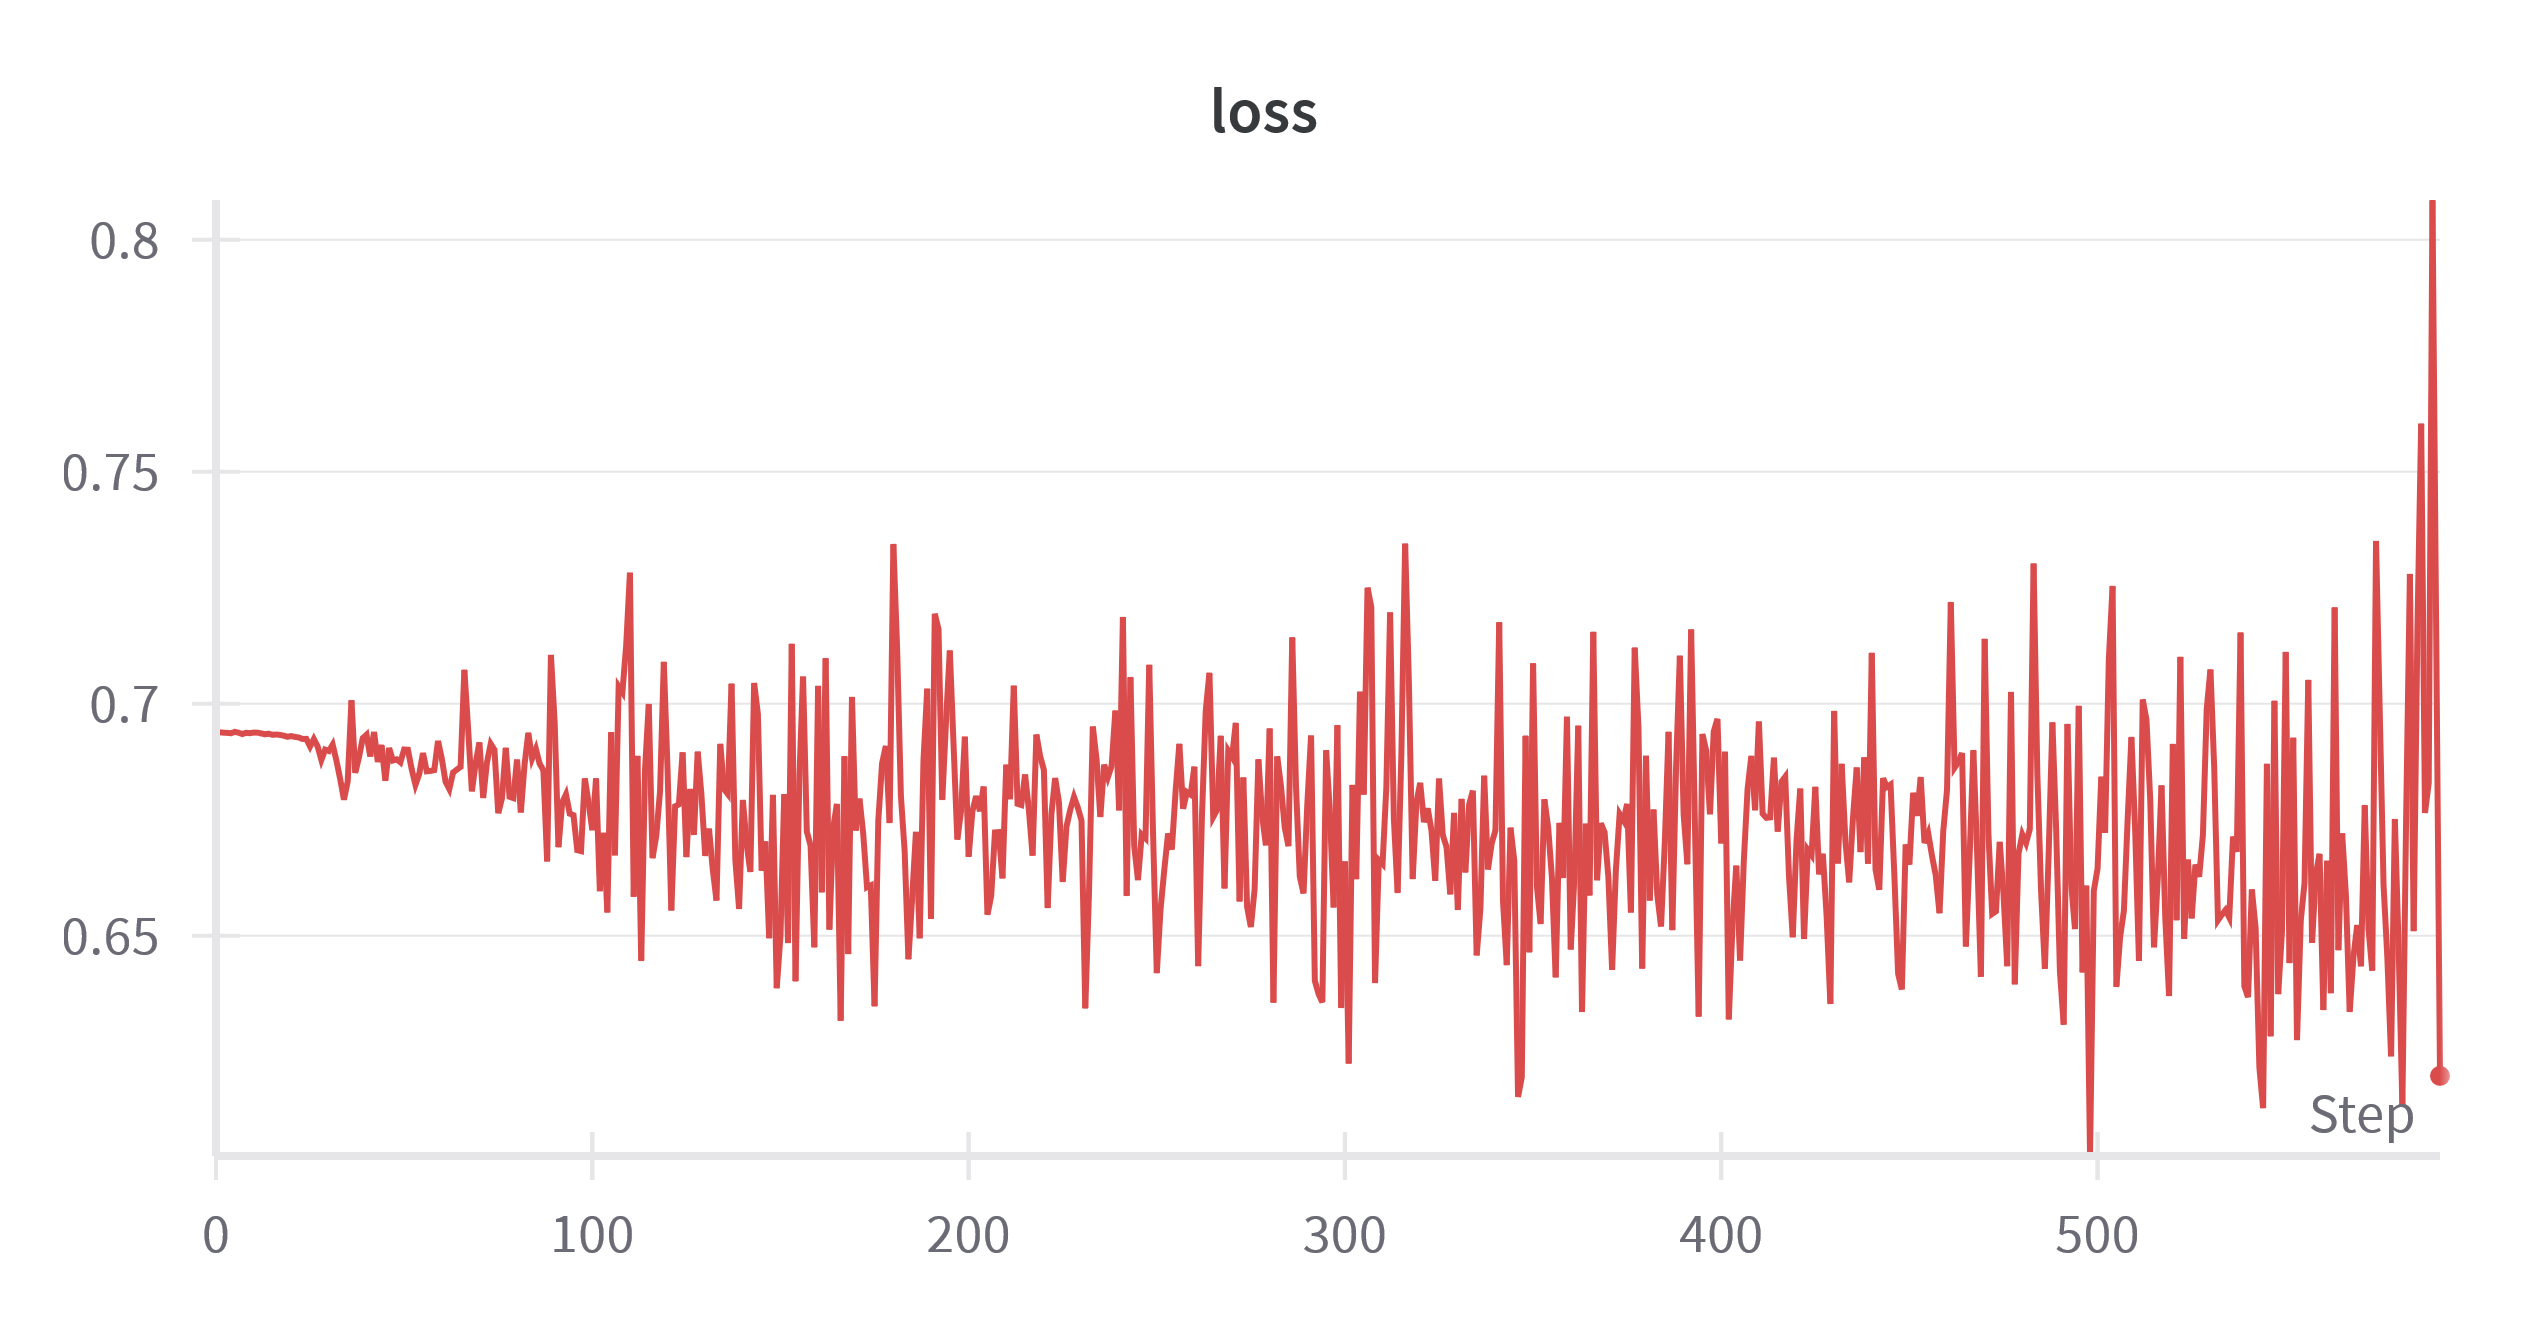
\includegraphics[width=1\linewidth]{figures/Figure17.png}
    \caption{Loss graph
    \textcolor{green}{chiar daca ai zis deja in text, e bine sa rezumi in caption info despre: modelul folosit pt a obtine aceste rezultate si datele (train sau test) pt care s-a calculat aceasta performanta}
    }
    \label{fig:fig16}
\end{figure}

\begin{figure}[!ht]
    \centering
    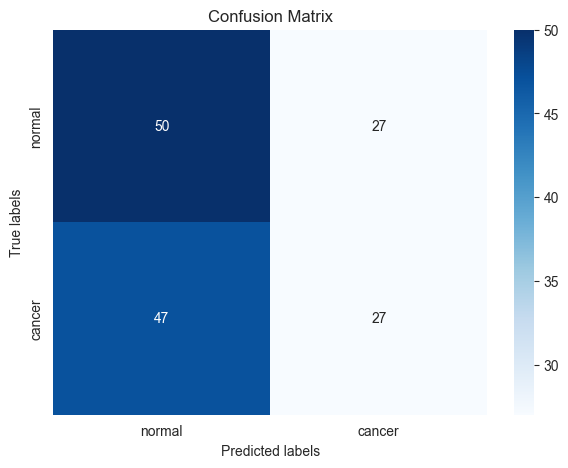
\includegraphics[width=0.5\linewidth]{figures/Figure18.png}
    \caption{Performance after 3 epochs
    \textcolor{green}{chiar daca ai zis deja in text, e bine sa rezumi in caption info despre: modelul folosit pt a obtine aceste rezultate si datele (train sau test) pt care s-a calculat aceasta performanta}
    }
    \label{fig:fig17}
\end{figure}

I resized the images to be 300$\times$300 and instead of adding the slices as channels of the same image, I added the slices as individual inputs. In doing so, I transformed a 568-length dataset into a 2,840-length one, and used a batch size of 64.


Upon figuring out the number of learnable parameters, which was around 3 milions, I wanted to increase the length of the dataset even more. With this purpose in mind I considered 22 slices of each input, and adding each of them individually resulted in a 12,496-length dataset.

Additionaly, I wanted to compare the loss of the two auxiliary models that GoogLeNet has to offer with the main output that it returns. In doing so, I returned to the initial implementation for the forward-pass method. However, I made a mistake in that I forgot that the original implementation doesn't include either activation function on the last layer, instead adding one only for the main output, not for the two auxiliary modules. Curiously, these two modules proved to obtain the lowest loss of all the experiments I performed, as shown in figure \ref{fig:fig18}.

\begin{figure}[!ht]
    \centering
    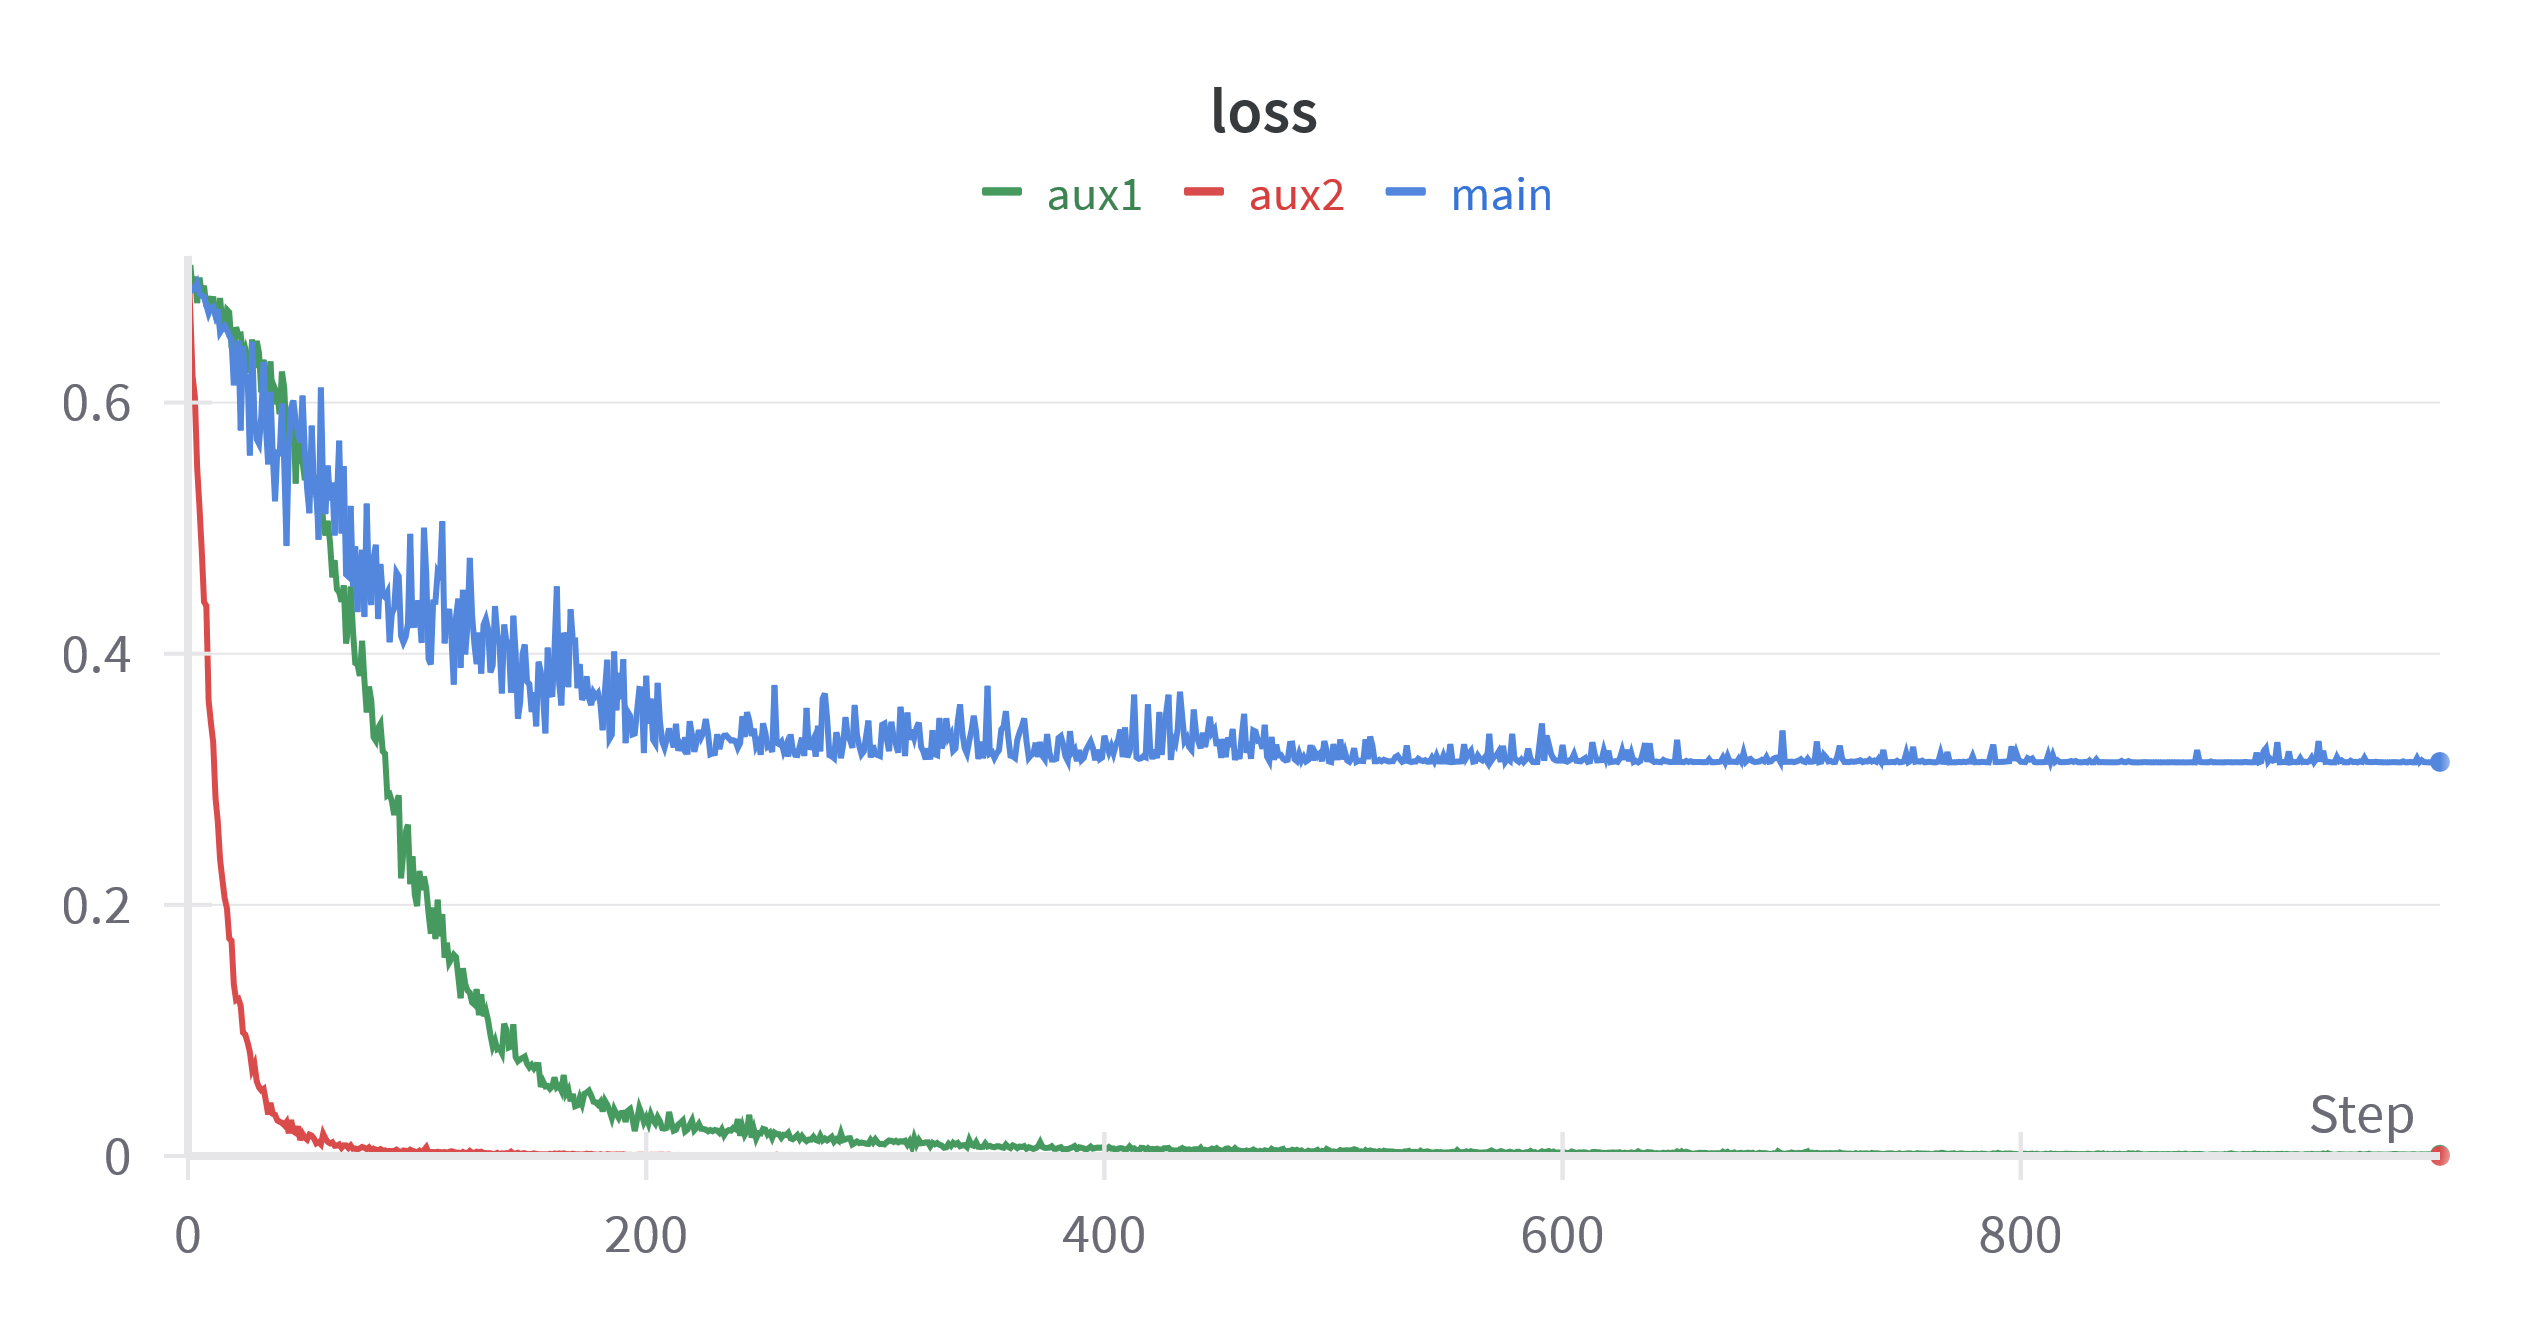
\includegraphics[width=1\linewidth]{figures/Figure19.png}
    \caption{Loss graph
    \textcolor{green}{chiar daca ai zis deja in text, e bine sa rezumi in caption info despre: modelele folosite pt a obtine aceste rezultate si datele (train sau test) pt care s-a calculat aceasta performanta}
    }
    \label{fig:fig18}
\end{figure}

Even with all these experiments and improvements, the best accuracy I managed to obtain was 0.5409
\textcolor{green}{tb indicat in care setup s-a obtinut acest scor}
.

\subsection{Experiment 5}

Towards the end of the process of training the classification model, I decided to use already trained weights from the Torchvision library.
\textcolor{green}{tot pe arhitectura GoogleLeNet? cea main sau aux1 sau aux2?} 
These weights had been trained on images from ImageNet.
\textcolor{green}{se precizeaza si cate imagini s-au folosit in acest pre-training si cat de mari au fost? Daca da, ar fi bine sa adaugi aceste detalii si aici (pot fi un reper util de ce acest model are loss asa mic fata de modelele antrenatede tine, dar pe seturi mult mai mici de imagini)} 
I also resized the images again and made them 512x512 in order to also fit the detection model. Figure \ref{fig:fig19} shows the loss graph after training the model for 5 epochs
\textcolor{green}{eu as zice ca de fapt e un fine-tunning a modelului pre-antrenat (pe ImageNet) pentru imaginile de breast cancer}
, while figure \ref{fig:fig20} shows the confusion matrix at the end of those epochs.

\begin{figure}[!ht]
    \centering
    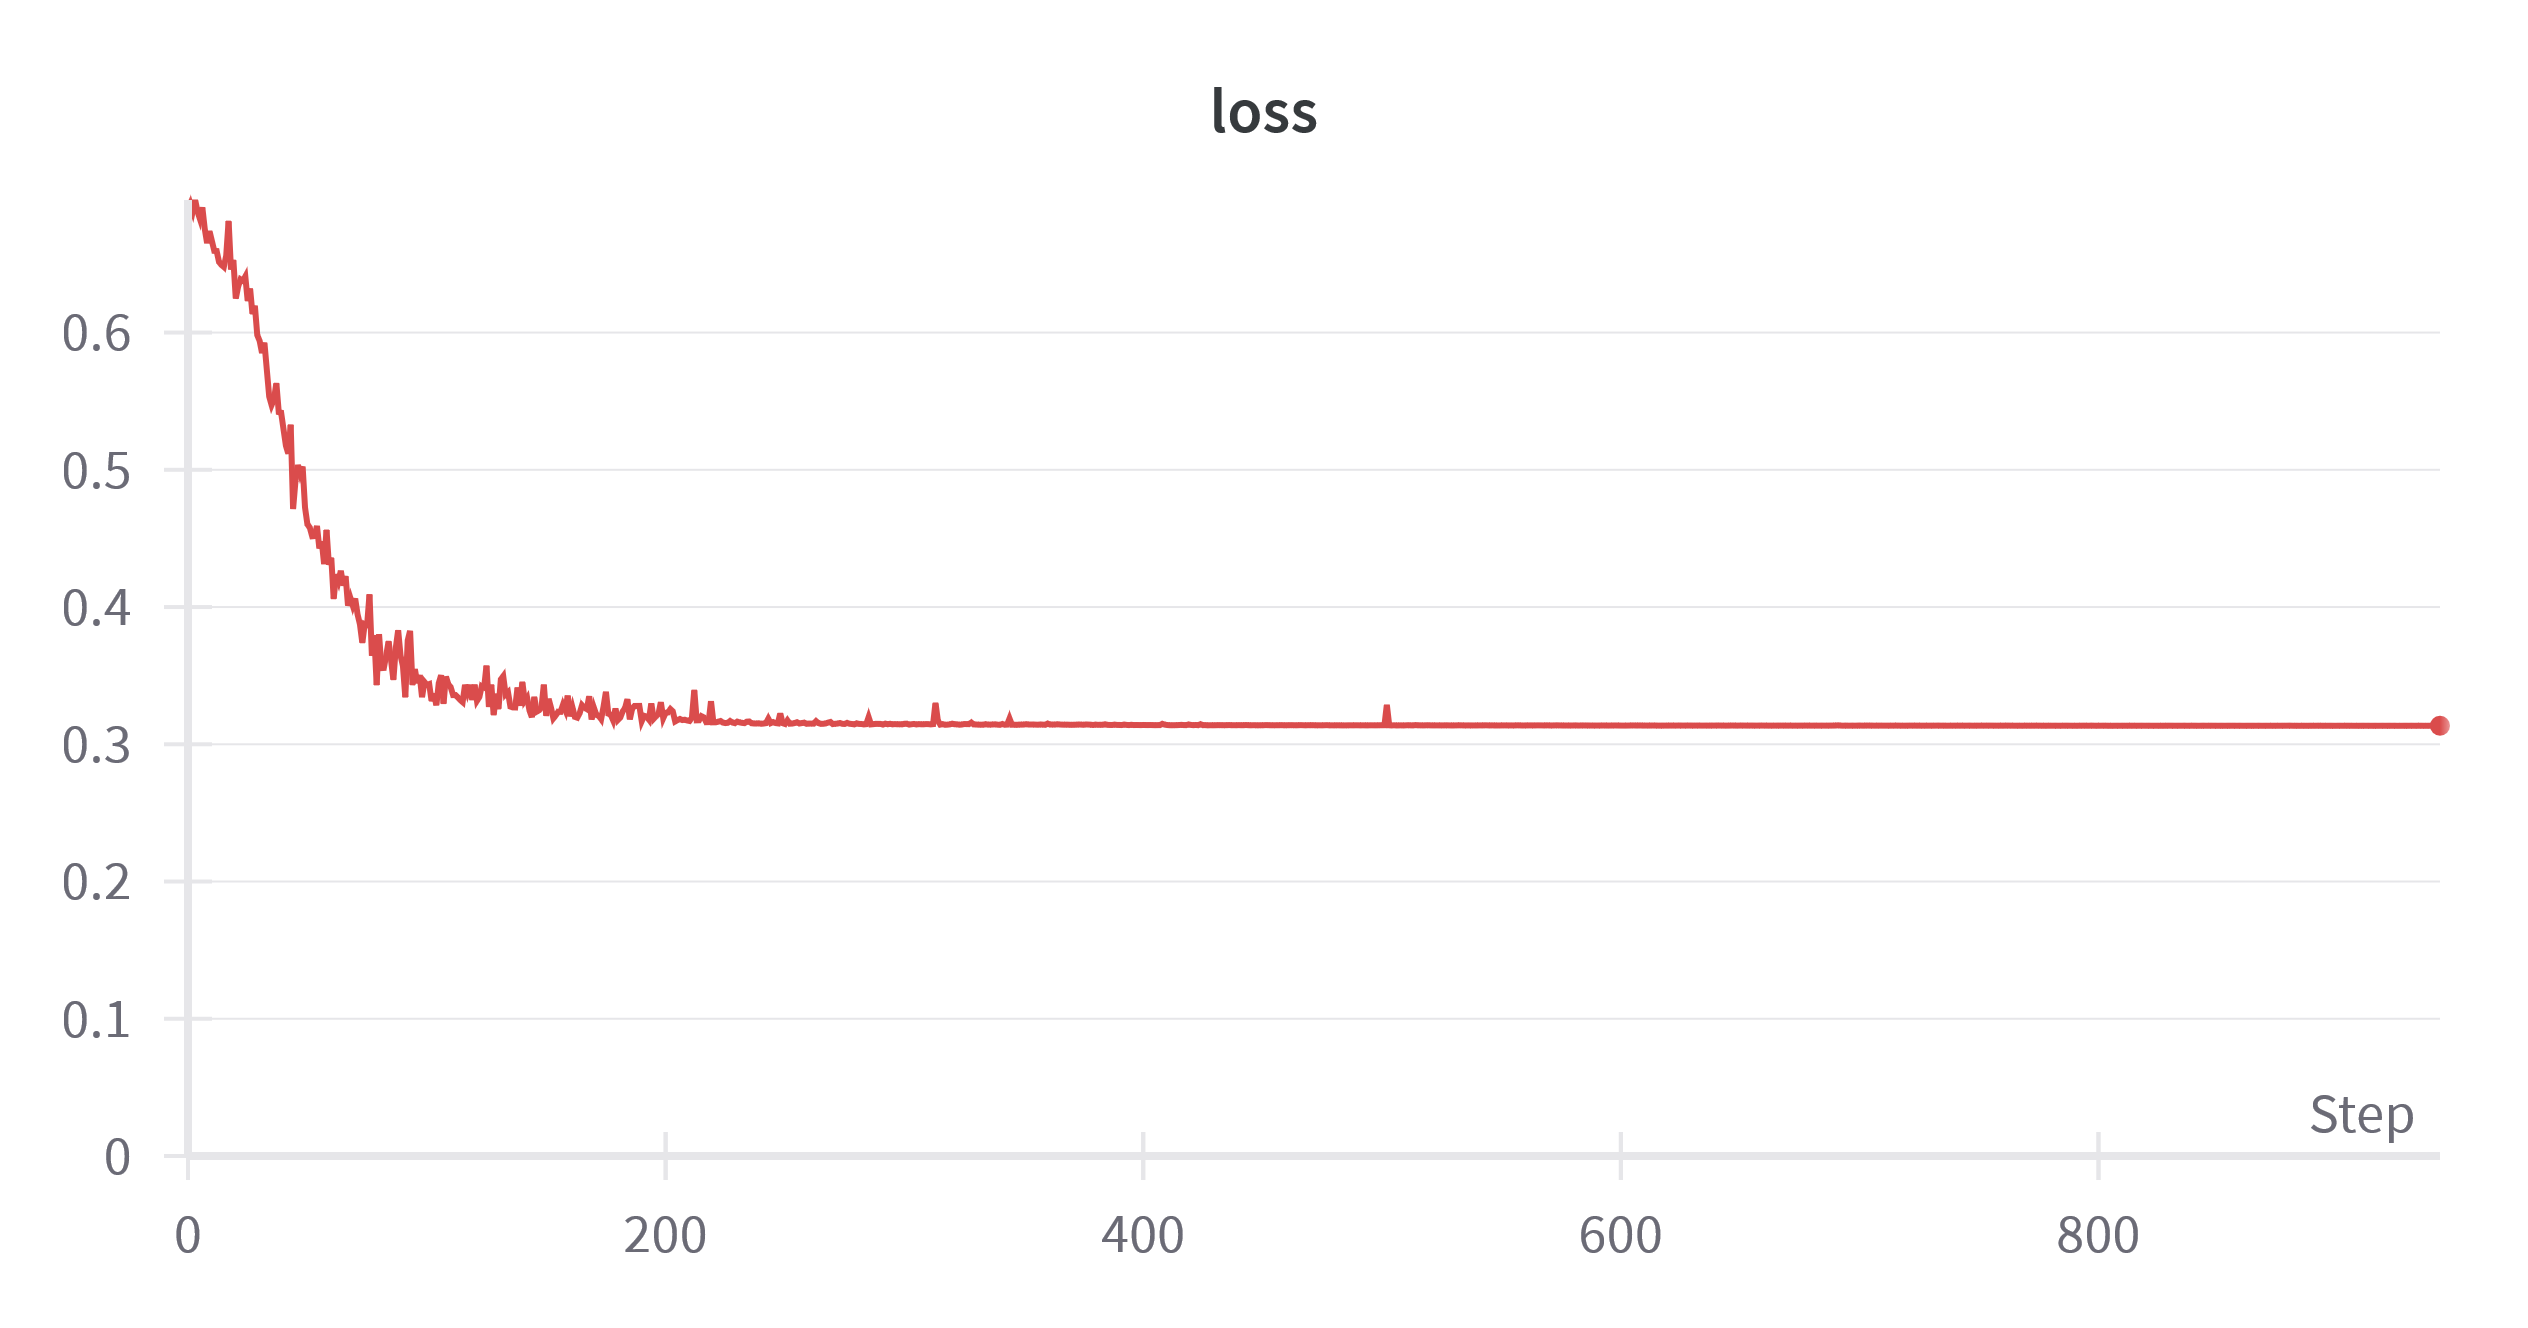
\includegraphics[width=1\linewidth]{figures/Figure20.png}
    \caption{Loss graph
    \textcolor{green}{chiar daca ai zis deja in text, e bine sa rezumi in caption info despre: modelul folosit pt a obtine aceste rezultate si datele (train sau test) pt care s-a calculat aceasta performanta}
    }
    \label{fig:fig19}
\end{figure}

\begin{figure}[!ht]
    \centering
    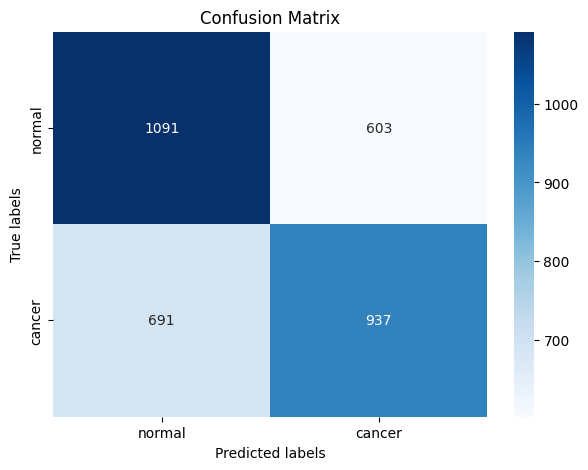
\includegraphics[width=0.5\linewidth]{figures/Figure21.png}
    \caption{Performance after epoch 5
    \textcolor{green}{chiar daca ai zis deja in text, e bine sa rezumi in caption info despre: modelul folosit pt a obtine aceste rezultate si datele (train sau test) pt care s-a calculat aceasta performanta}
    }
    \label{fig:fig20}
\end{figure}

I also experimented with different batch sizes for the model.
\textcolor{green}{cel cu weights pre-trained pe ImageNet?}  
Therefore, I trained the model with the same configuration as the previous run, except I modified the size of the batches from 64 to 128. Figure \ref{fig:fig21} shows the comparison in loss between these two experiments. This second model I also trained for 5 epochs; however, the difference in steps in the graph comes from increasing the number of inputs in each batch, which means fewer batches over the dataset and overall fewer steps.

\begin{figure}[!ht]
    \centering
    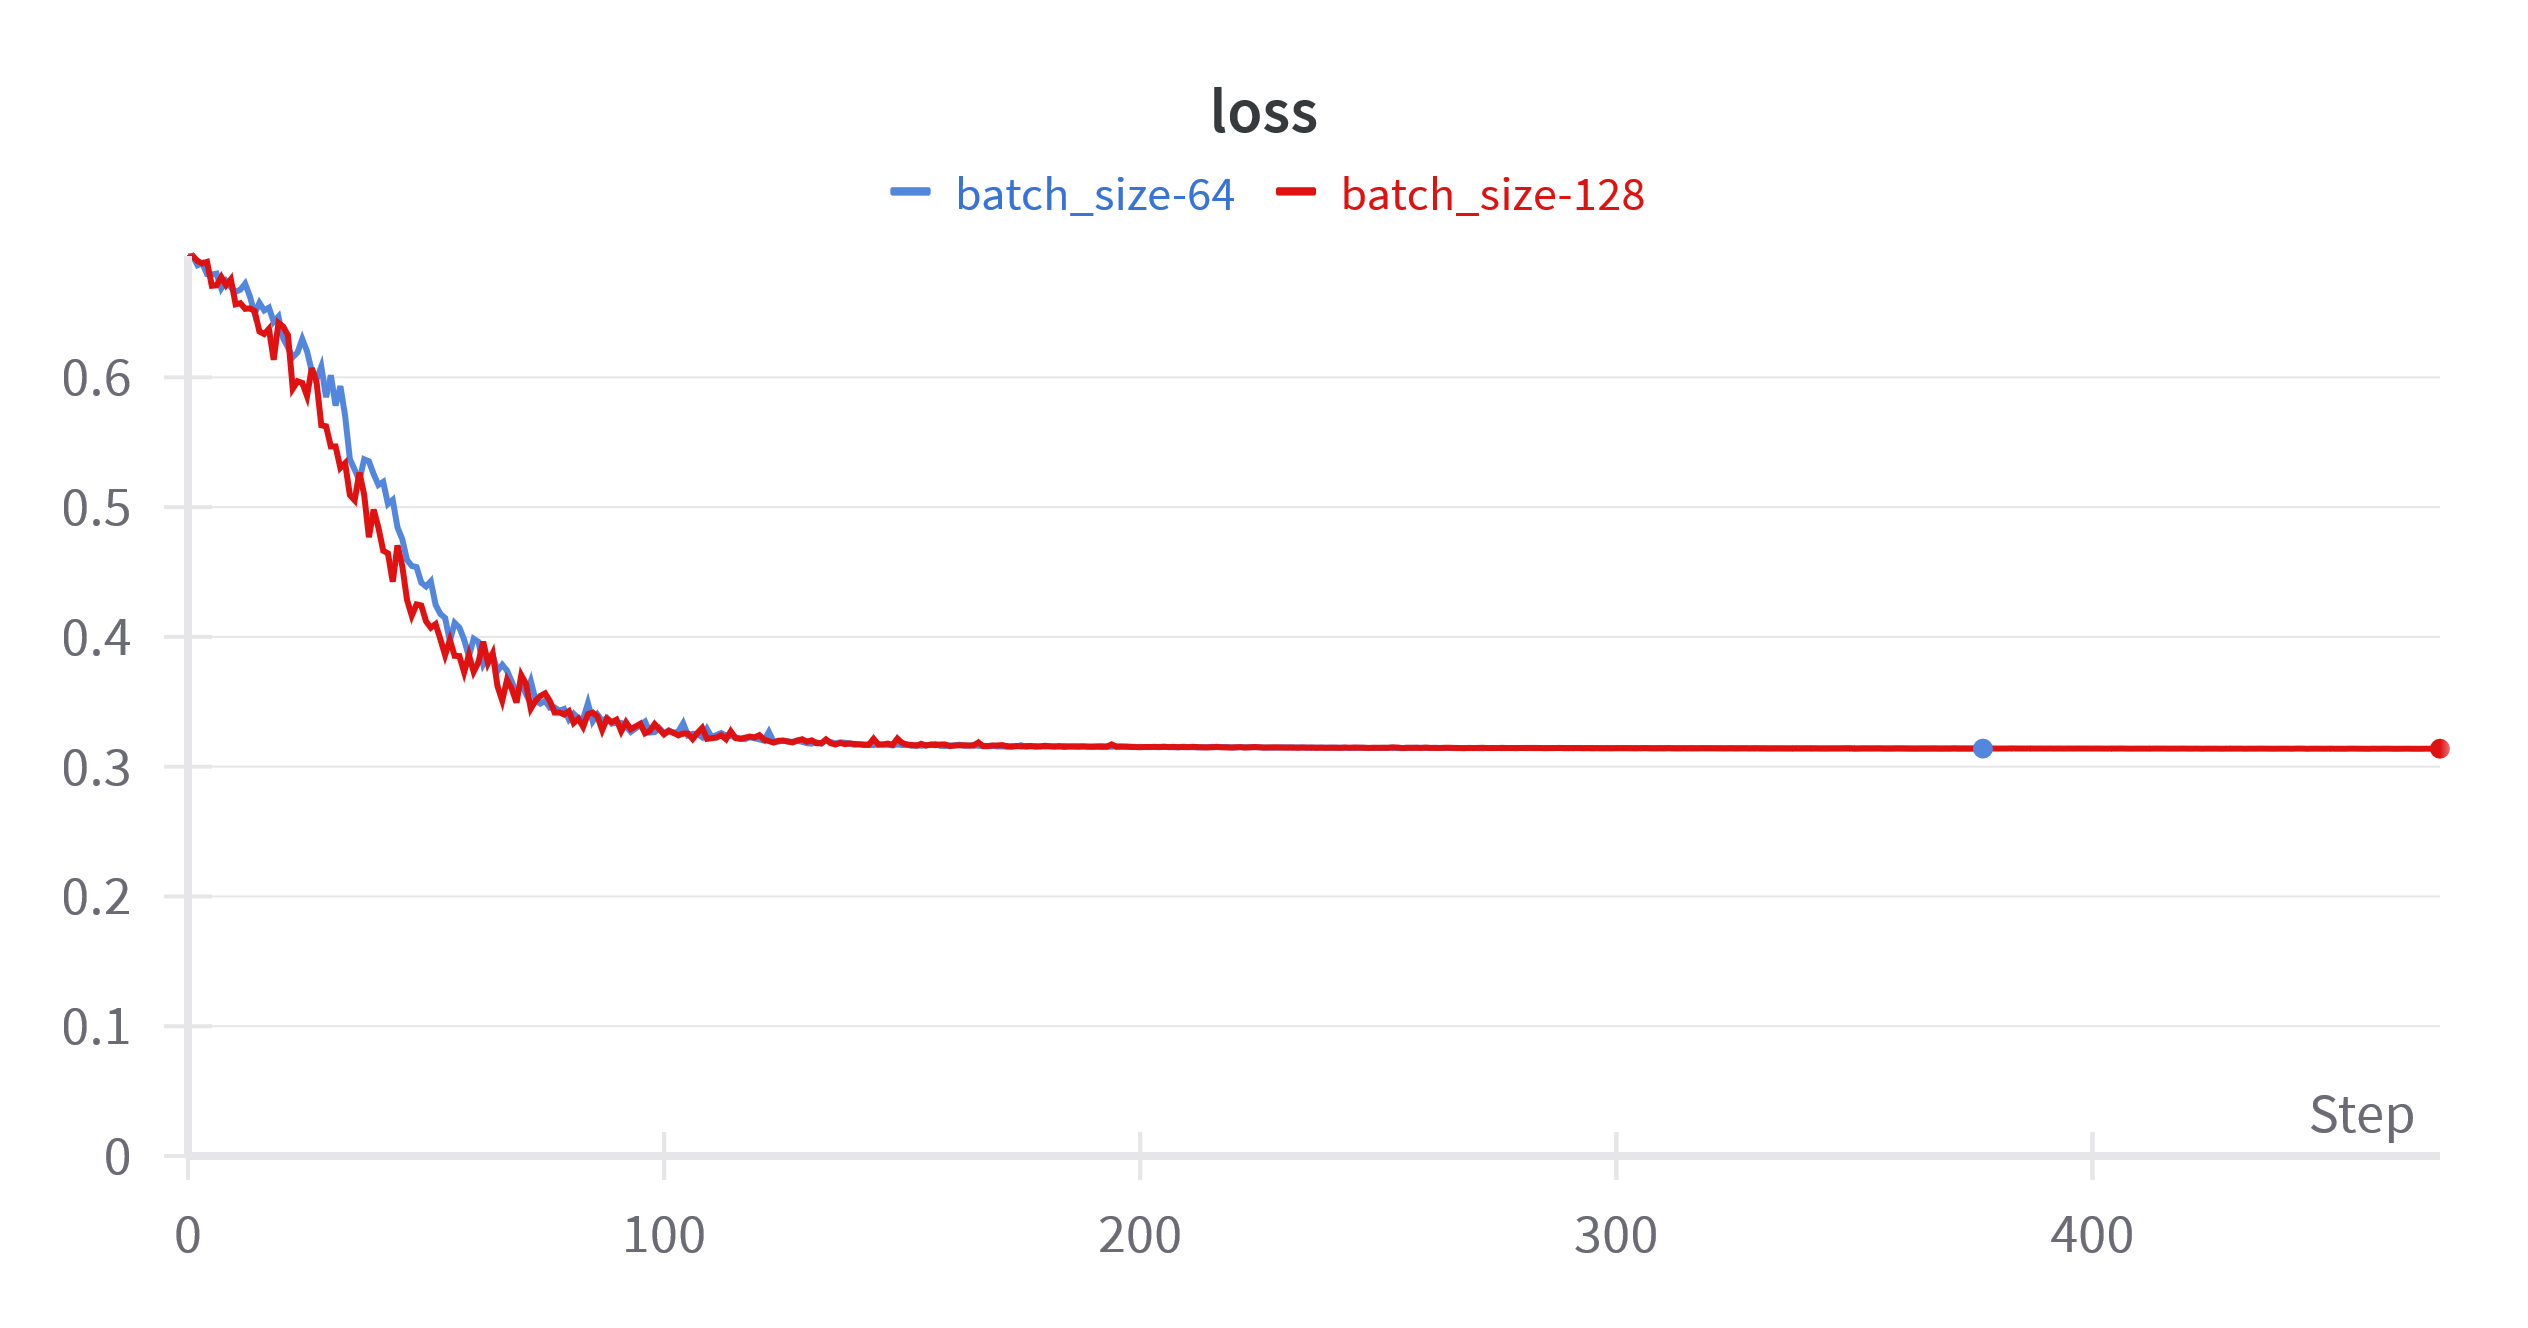
\includegraphics[width=1\linewidth]{figures/Figure22.png}
    \caption{Loss graph
    \textcolor{green}{chiar daca ai zis deja in text, e bine sa rezumi in caption info despre: modelul folosit pt a obtine aceste rezultate si datele (train sau test) pt care s-a calculat aceasta performanta}}
    \label{fig:fig21}
\end{figure}

The final configuration that I came to included: batches of size 128, pre-trained weights trained with images from ImageNet, a learning rate of 0.0001, learning rate decay using the StepLR implementation with a step size of 5 and gamma of 0.1, an image size of 512, and 22 inputs of each image representing different slices from the 3D scans. The loss obtained using a learning rate of Step instead of Exponential is shown in figure \ref{fig:fig22}.

\begin{figure}[!ht]
    \centering
    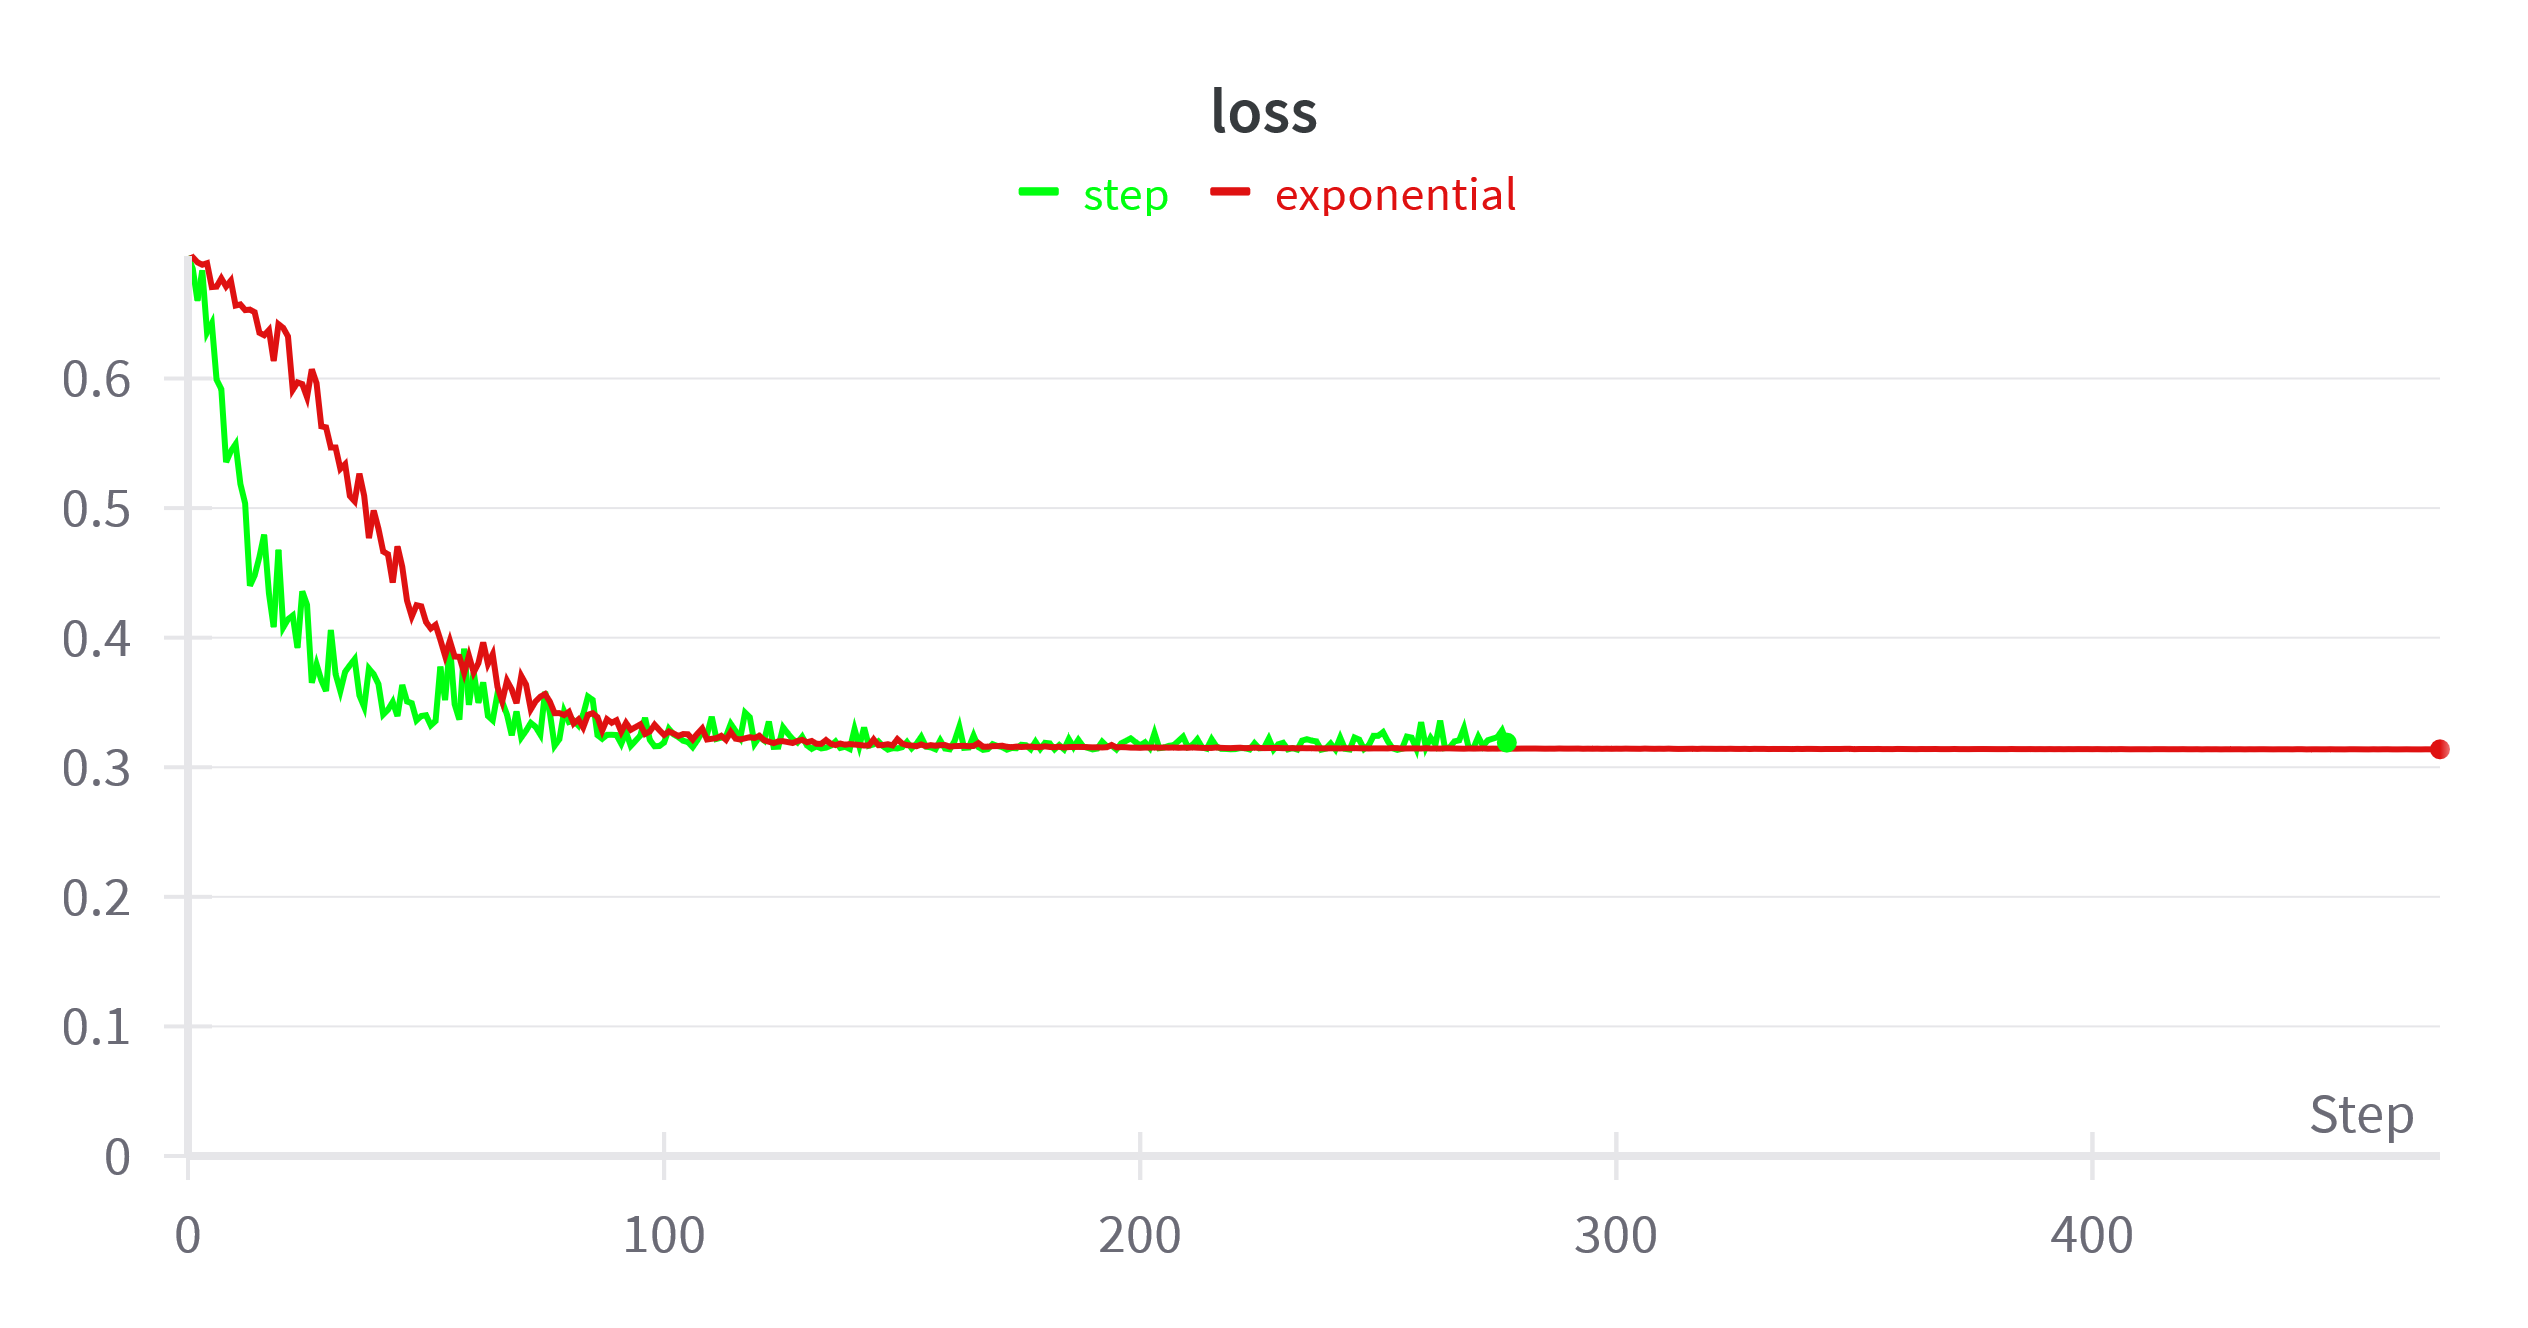
\includegraphics[width=1\linewidth]{figures/Figure24.png}
    \caption{Loss graph
    \textcolor{green}{chiar daca ai zis deja in text, e bine sa rezumi in caption info despre: modelele folosite pt a obtine aceste rezultate si datele (train sau test) pt care s-a calculat aceasta performanta}
    }
    \label{fig:fig22}
\end{figure}

\textcolor{green}{eu as adauga si la acest model matricea de confuzie}


\begin{table}[!ht]
    \centering
    \begin{tabular}{|c|c|c|c|c|c|c|}
        \hline
        Experiment & \#classes & Image size & Model & trained/pre-trained & (hyper)params & Performance (Acc) \\
        \hline\hline
        Exp1 & 4 & 5$\times$2457$\times$1890 & GoogleLeNet & trained & ? & ?\\
        \hline
        Exp2 & 4 & 5$\times$2457$\times$1890 & aux1 & trained & ? & ?\\
        \hline
        Exp3 & 4 & 5$\times$2457$\times$1890 & aux2 & trained & ? & ?\\
        \hline
        Exp4 & 2 & 1$\times$300$\times$300 & ? & trained & ? & ?\\
        \hline
        Exp5 & 2 & 1$\times$300$\times$300 & ? & pre-trained & ? & ?\\
        \hline    
    \end{tabular}
    \caption{Classification models}
    \label{tab:classificationModels}
\end{table}


\section{Detection experiments}

\textcolor{green}{aici ar fi bine sa fie mai intai o scurta poveste legata de flow: ca dupa ce au fost clasificate imaginile, ai vrut sa vezi daca poti detecta si localiza tumori in aceste imagini. De aceea, ai folosit doar imaginile cu tumori (asa-i?) pe care ai aplicat un algoritm de detectie.}

\textcolor{green}{din nou, le-as lua pe rand:
0. datele folosite (cate imagini, cat de mari, cate slice-uri, cate tumori sunt in ele, cum sunt distribuite tumori in train si test, daca te-ai dus pe varianta ca inputul e o singura felie sau mai multe felii)\\
1. detalii despre algoritmul de detectie - arhitectura si (hyper)param\\
2. evolutia loss-ului pe train (eventual si pe test)\\
3. performanta pe datele de test\\}

\subsection{Experiment 1}


In the first implementation of this run, I opted to not use pre-trained weights in order to compare the proper results. With that purpose in mind, the first configuration included a learning rate of 0.0001 and a learning rate decay of ReduceLROnPlateau, with the minimum value for the learning rate being \(1e^{-8}\). However, this learning rate decay is only utilized after the test loop has finished running, and the metric used is the loss obtained for the test dataset. The number of slices used from each input remained at 22, as for the final configuration for the classification model, and the size of the batches was changed to 16. Considering the fact that the images were resized in order to be 512x512, I scaled the coordinates 
\textcolor{green}{of bounding boxes?} 
accordingly. Also, the configuration for the EfficientDet is the first one, D-0, as it has the same image size as the size for the inputs used by me. The attributes associated with the D-0 type EfficientDet were obtained by calling the proper function from the library Effdet. 
\textcolor{green}{tb amintit si ce fel de loss foloseste EfficNet-ul (pt ca la clasificare ai zis ca e Cross-entropy cu weight-uri, aici poti zice ca e doar CE simplu sau care loss l-ai folosit)}

\textcolor{green}{e ok ce ai zis, dar se amesteca putin ideile: incepi cu detalii despre model si param, apoi zici de date si sliece-uri, apoi iar de param (batch size), apoi iar de date (resize si scaling), apoi iar de param (configuratie model). Eu as incerca sa le grupez mai bine, sa nu sar de la un subiect la altul. Te poti ghida dupa cele 5 puncte pe care ti le-am dat mai sus.}

Figure \ref{fig:fig23} shows the loss for the train dataset and the test dataset. The big jumps from the steps in both graphs indicate that the missing steps are in the complementary graph. 
\textcolor{green}{oare la ce anume te referi?}

\begin{figure}[!ht]
    \subfigure[]{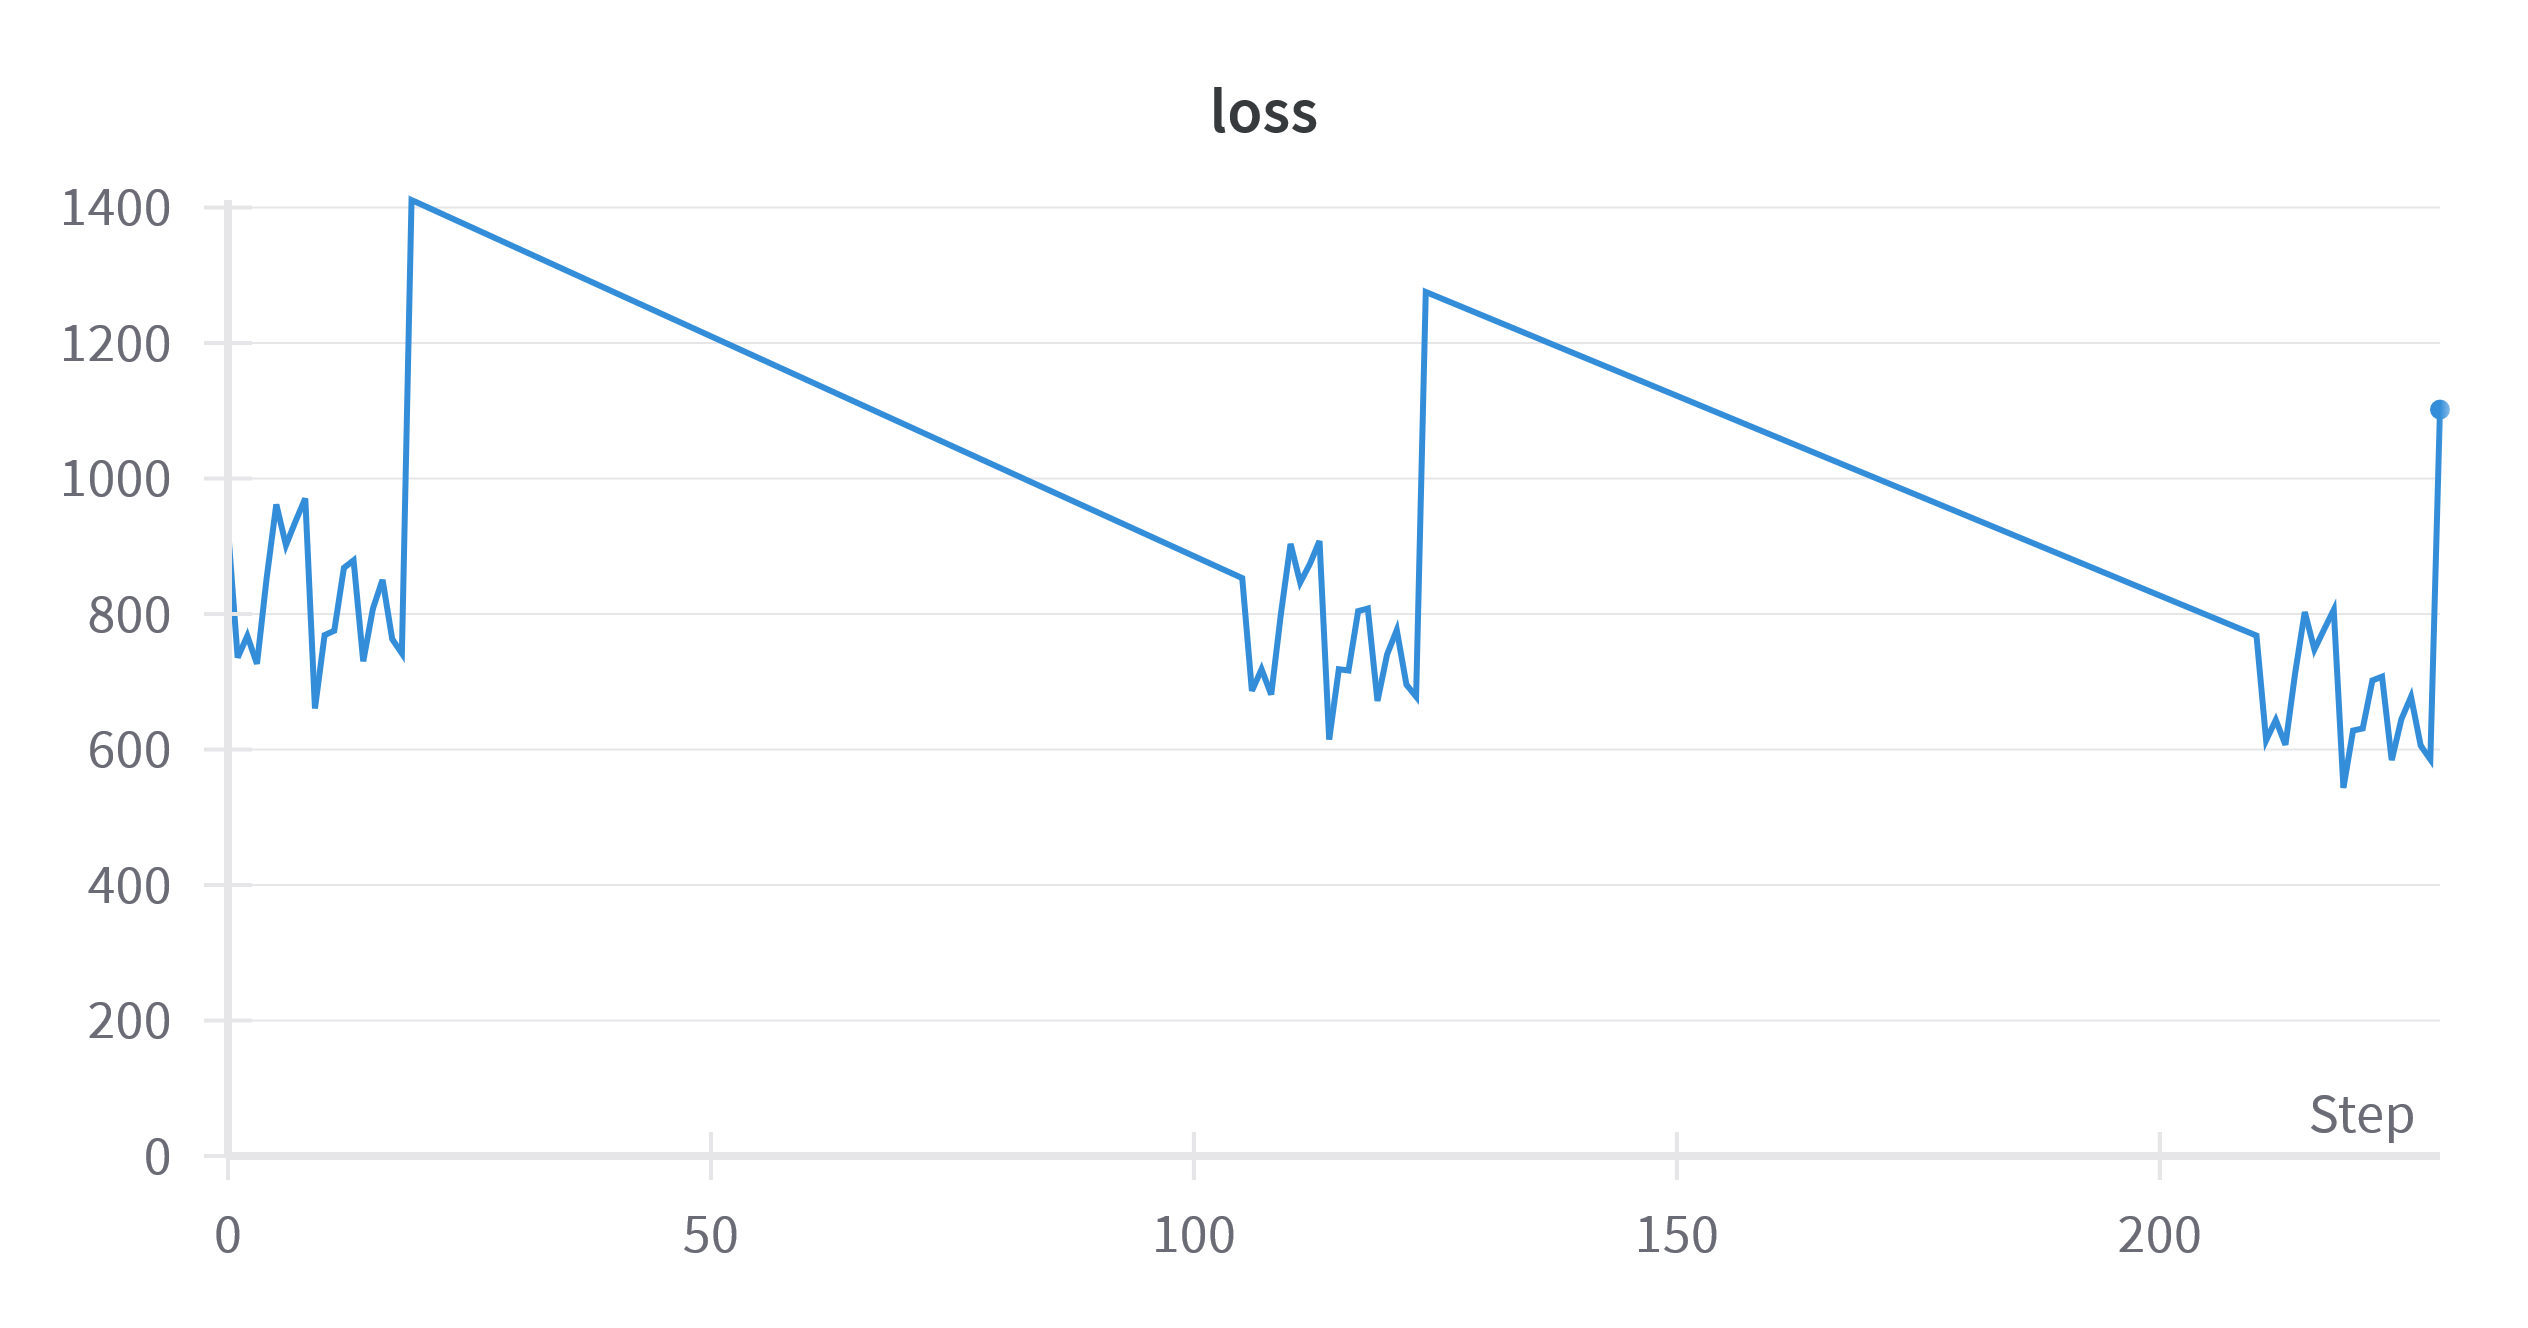
\includegraphics[width=0.45\linewidth]{figures/Figure25.png}}
    \subfigure[]{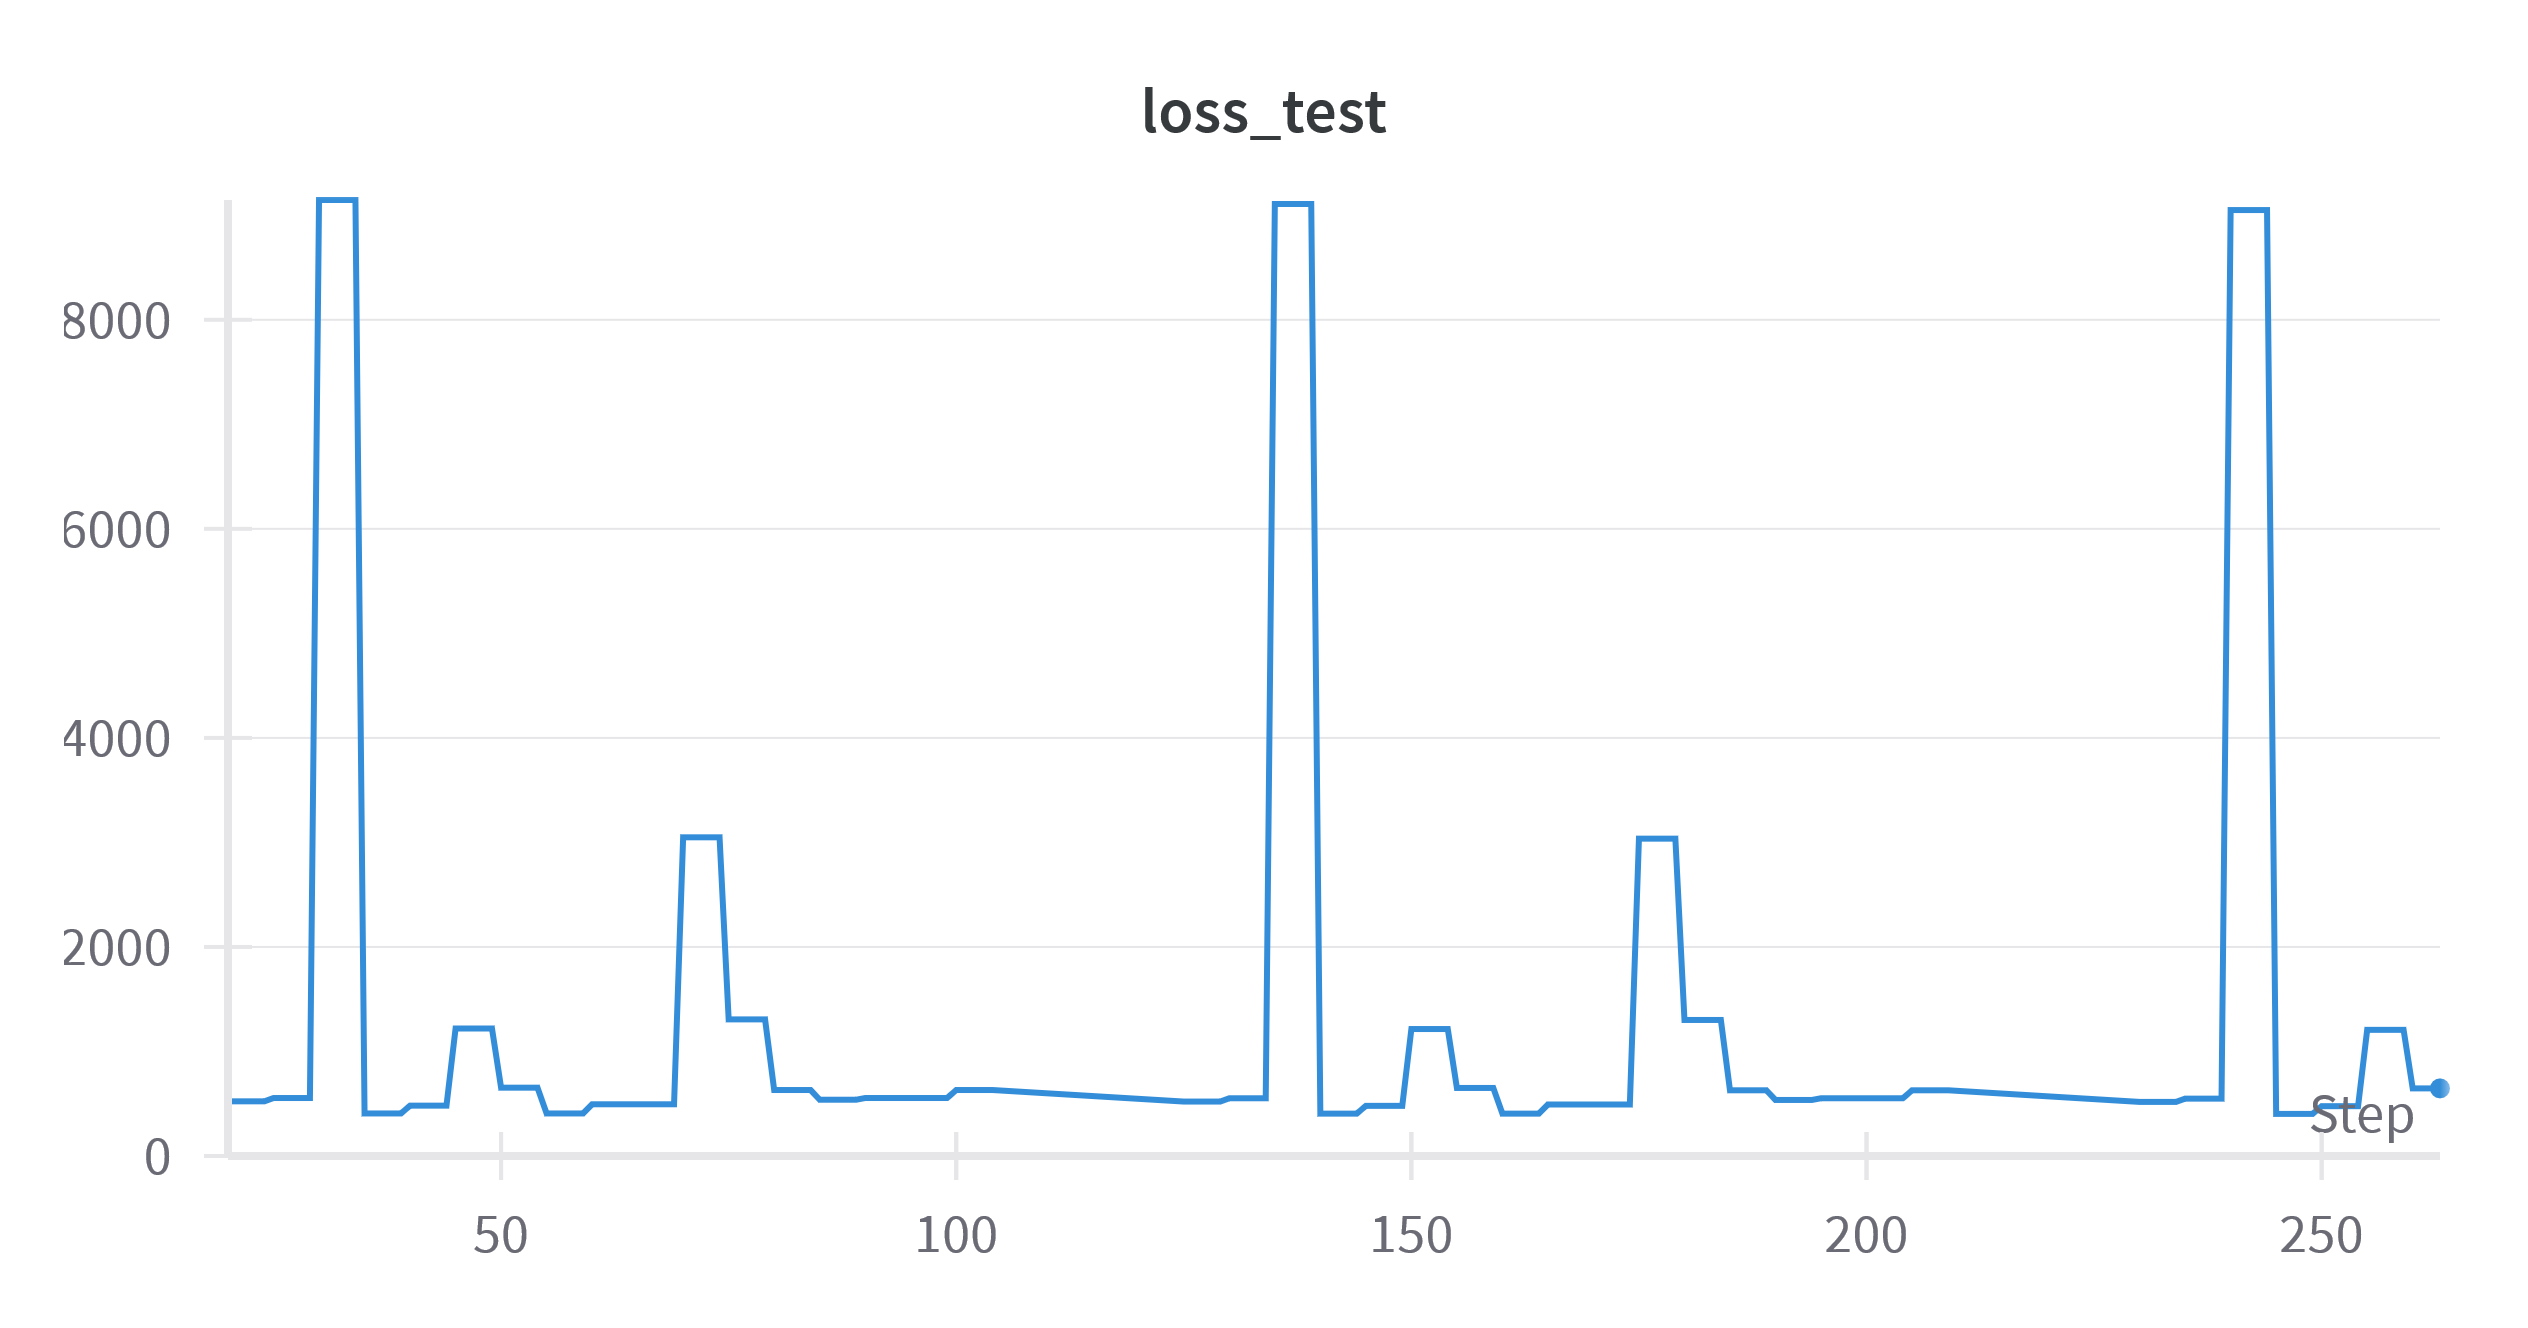
\includegraphics[width=0.45\linewidth]{figures/Figure26.png}}
    \caption{(a) Train loss (b) Test loss
    \textcolor{green}{tb adaugate info despre model si datele pe care s-au obtinut aceste rezultate}
    }
    \label{fig:fig23}
\end{figure}

\subsection{Experiment 2}

The figure does not indicate any loss reduction, so I changed the configuration of the detector. I chose not to normalize the images
\textcolor{green}{deci la ce dimensiune le-ai folosit?}
and test how the model behaves. I also discovered that EfficientDet works better when the bounding box coordinates are given in (y,x,y,x) order, and so I changed it from (x, y, width, height). Additionally, I used pre-trained weights, which I obtained from Alex Shonenkov's Kaggle account ~\cite{link6} and I reset the Head Nets in order to fit my classification problem. 
\textcolor{green}{doar head-ul de classificare sau ambele head-uri (atat pt regresie = BB, cat si pt calsificare (Ce ob e in BB)?)} 
I stopped the run before it had a chance to validate the model, so there is no graph for the test loss. Figure \ref{fig:fig24} shows the train loss.
\textcolor{green}{tb adaugate info despre setup-ul de antrenare a head-ului (learning rate, decay, optimizator, batch size, loss, no of epochs)}

\begin{figure}[!ht]
    \centering
    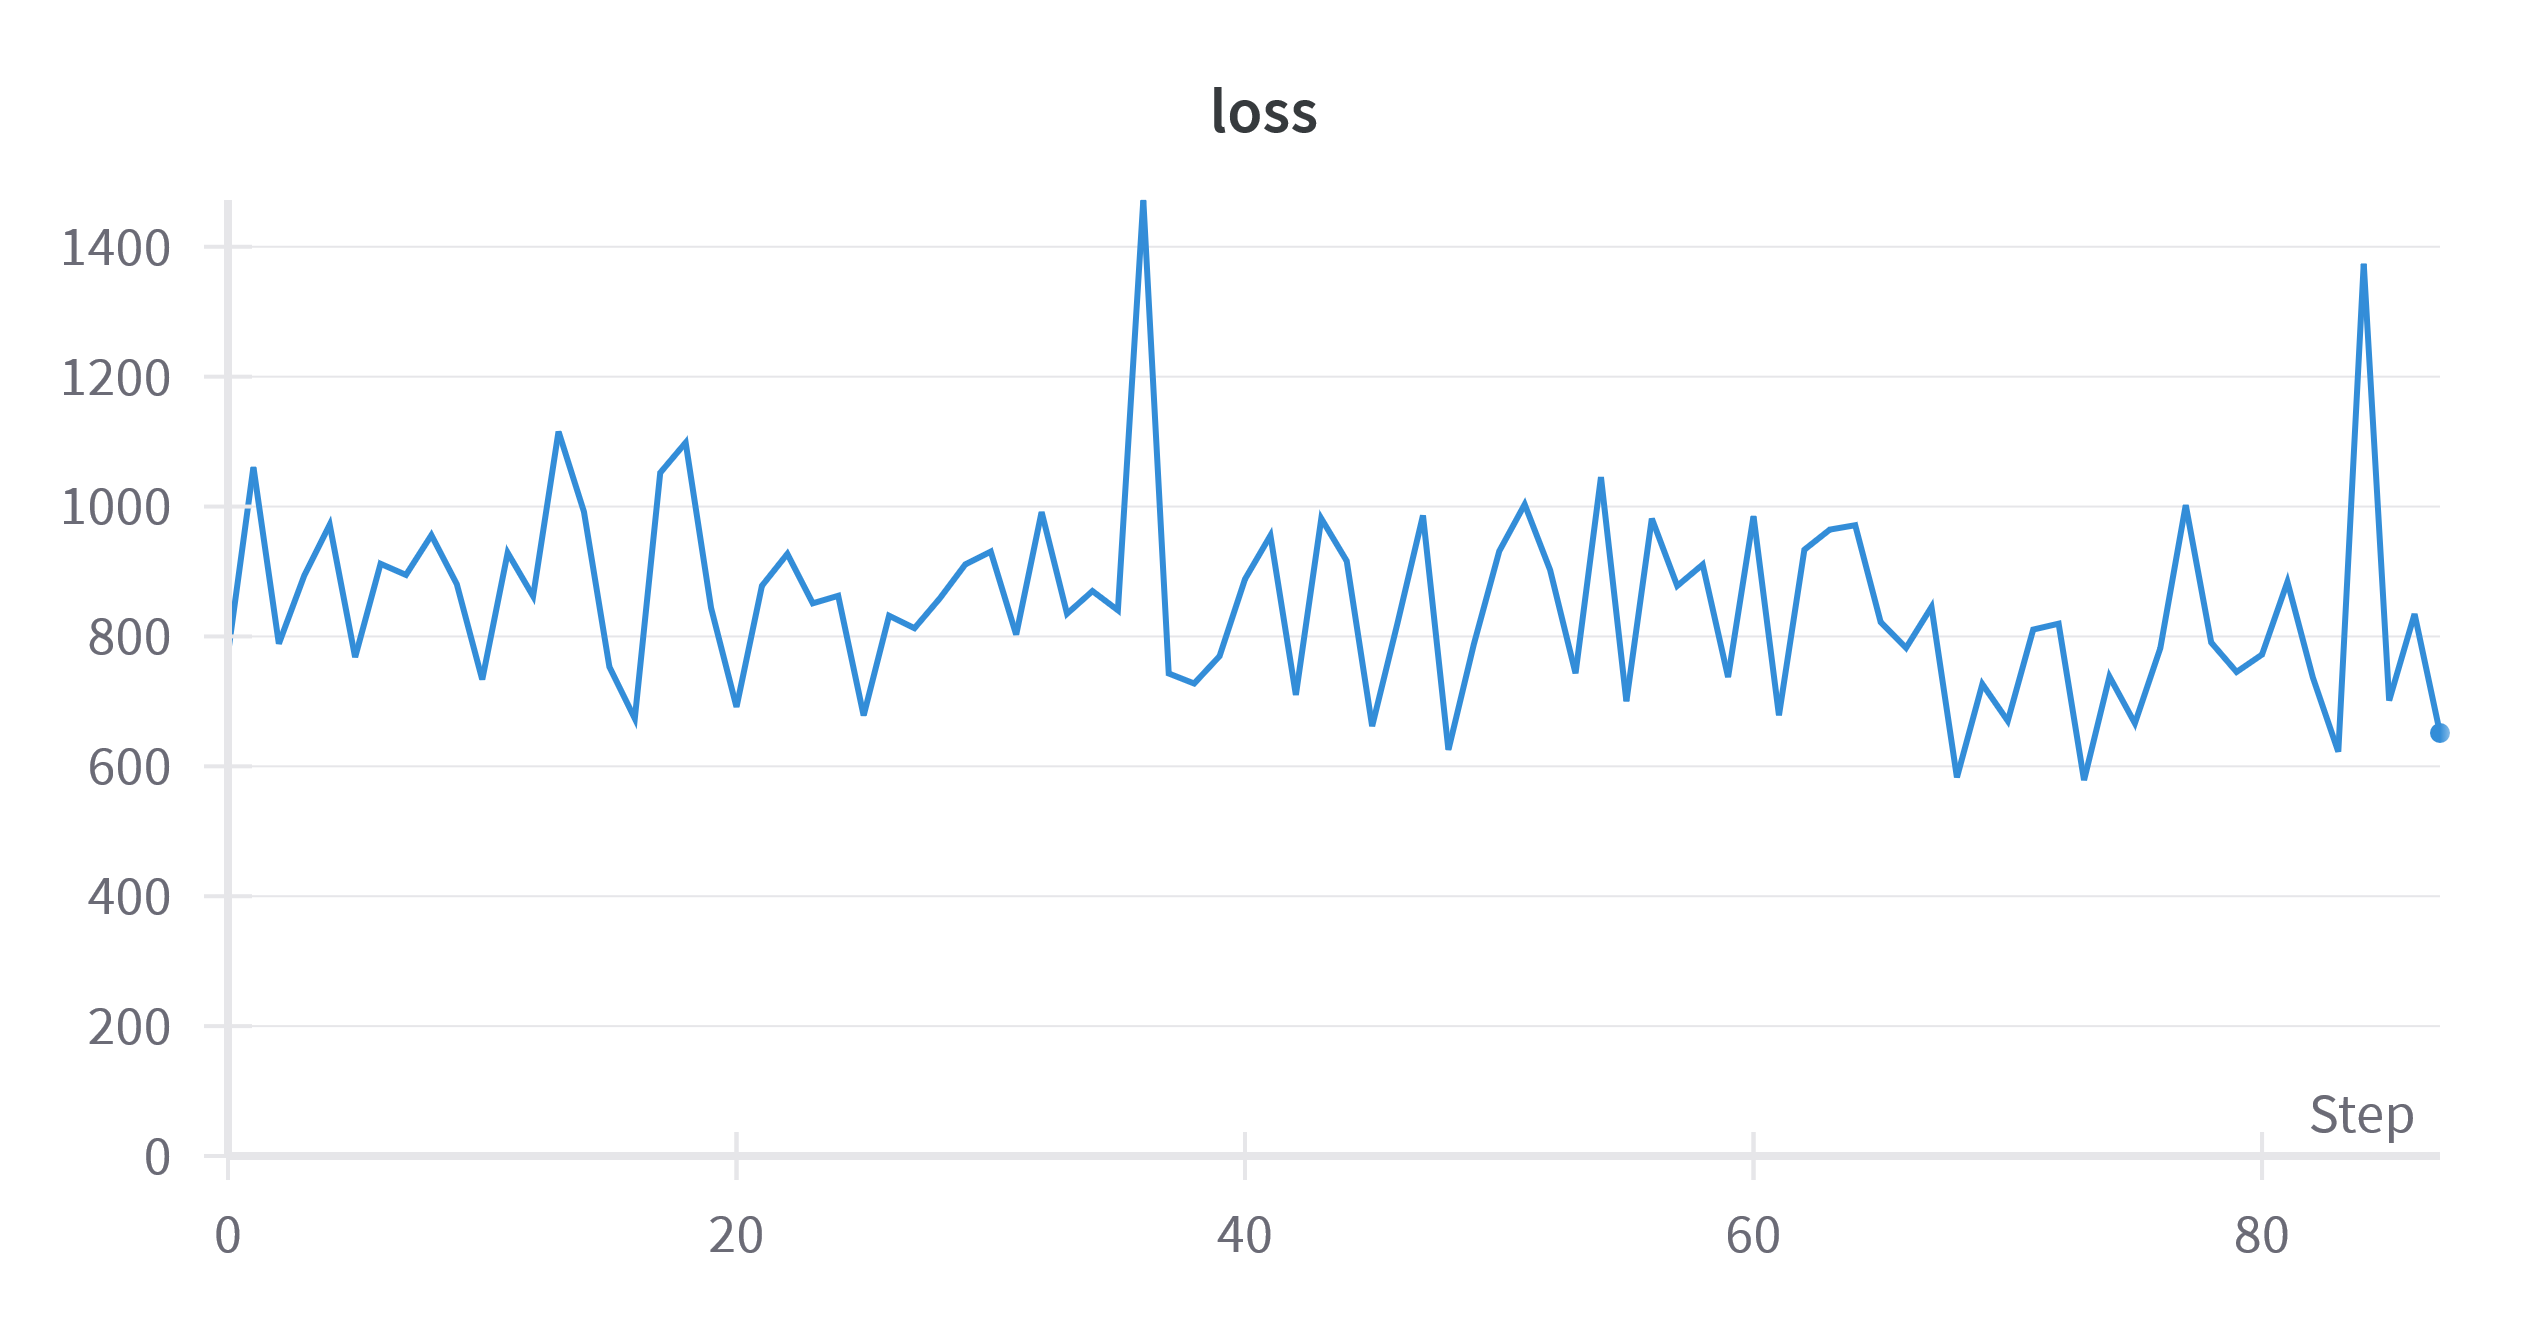
\includegraphics[width=1\linewidth]{figures/Figure27.png}
    \caption{Loss graph
    \textcolor{green}{tb adaugate info despre model si datele pe care s-au obtinut aceste rezultate}
    }
    \label{fig:fig24}
\end{figure}



I took the same configuration and trained it for 50 epochs to see how the loss evolved. Instead of running the run loop
\textcolor{green}{ce inseamna run loop? oare e training loop?} 
once for 50 epochs, I ran the loop five times with 10 epochs each. Because of this, the graph is not continuous; each batch of 10 epochs starts at the 0 step. 
\textcolor{green}{dar cu weight-urile deja invatate in loop-ul precedent?} 
In the first 10 epochs, shown in figure \ref{fig:fig25}, the loss decrease is steep, and so is the test loss. However, after 40 epochs, the decline gets more gradual, as shown in figure \ref{fig:fig26}.

\begin{figure}[!ht]
    \subfigure[]{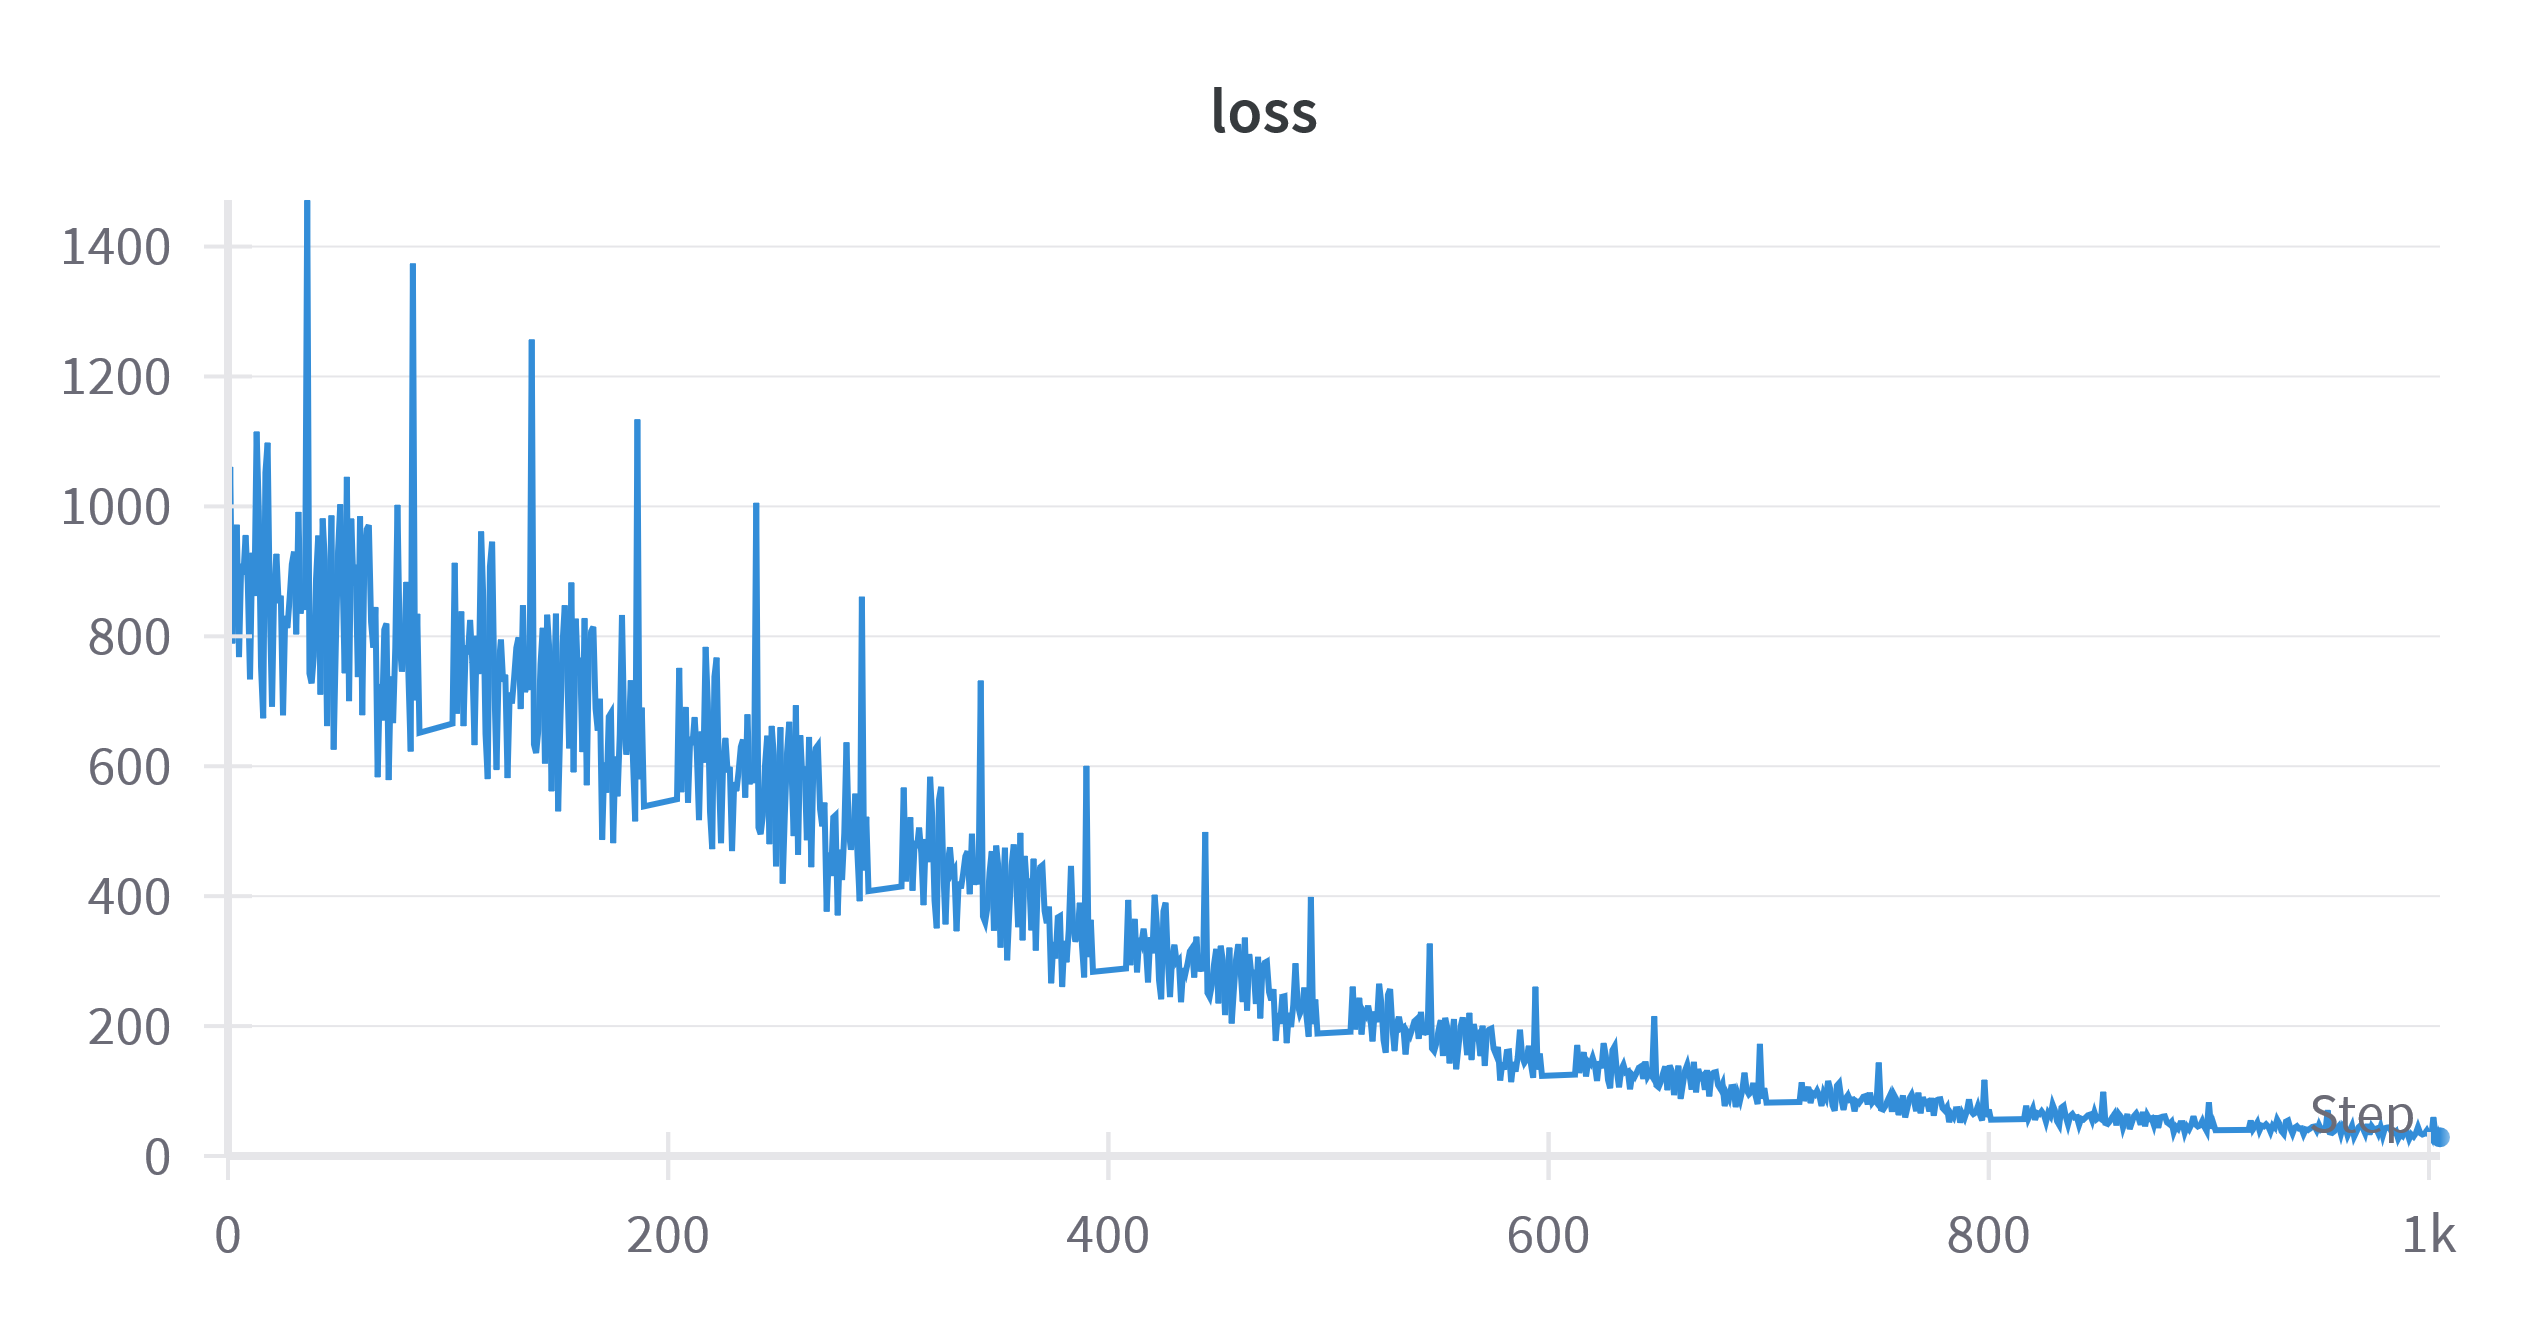
\includegraphics[width=0.45\linewidth]{figures/Figure28.png}}
    \subfigure[]{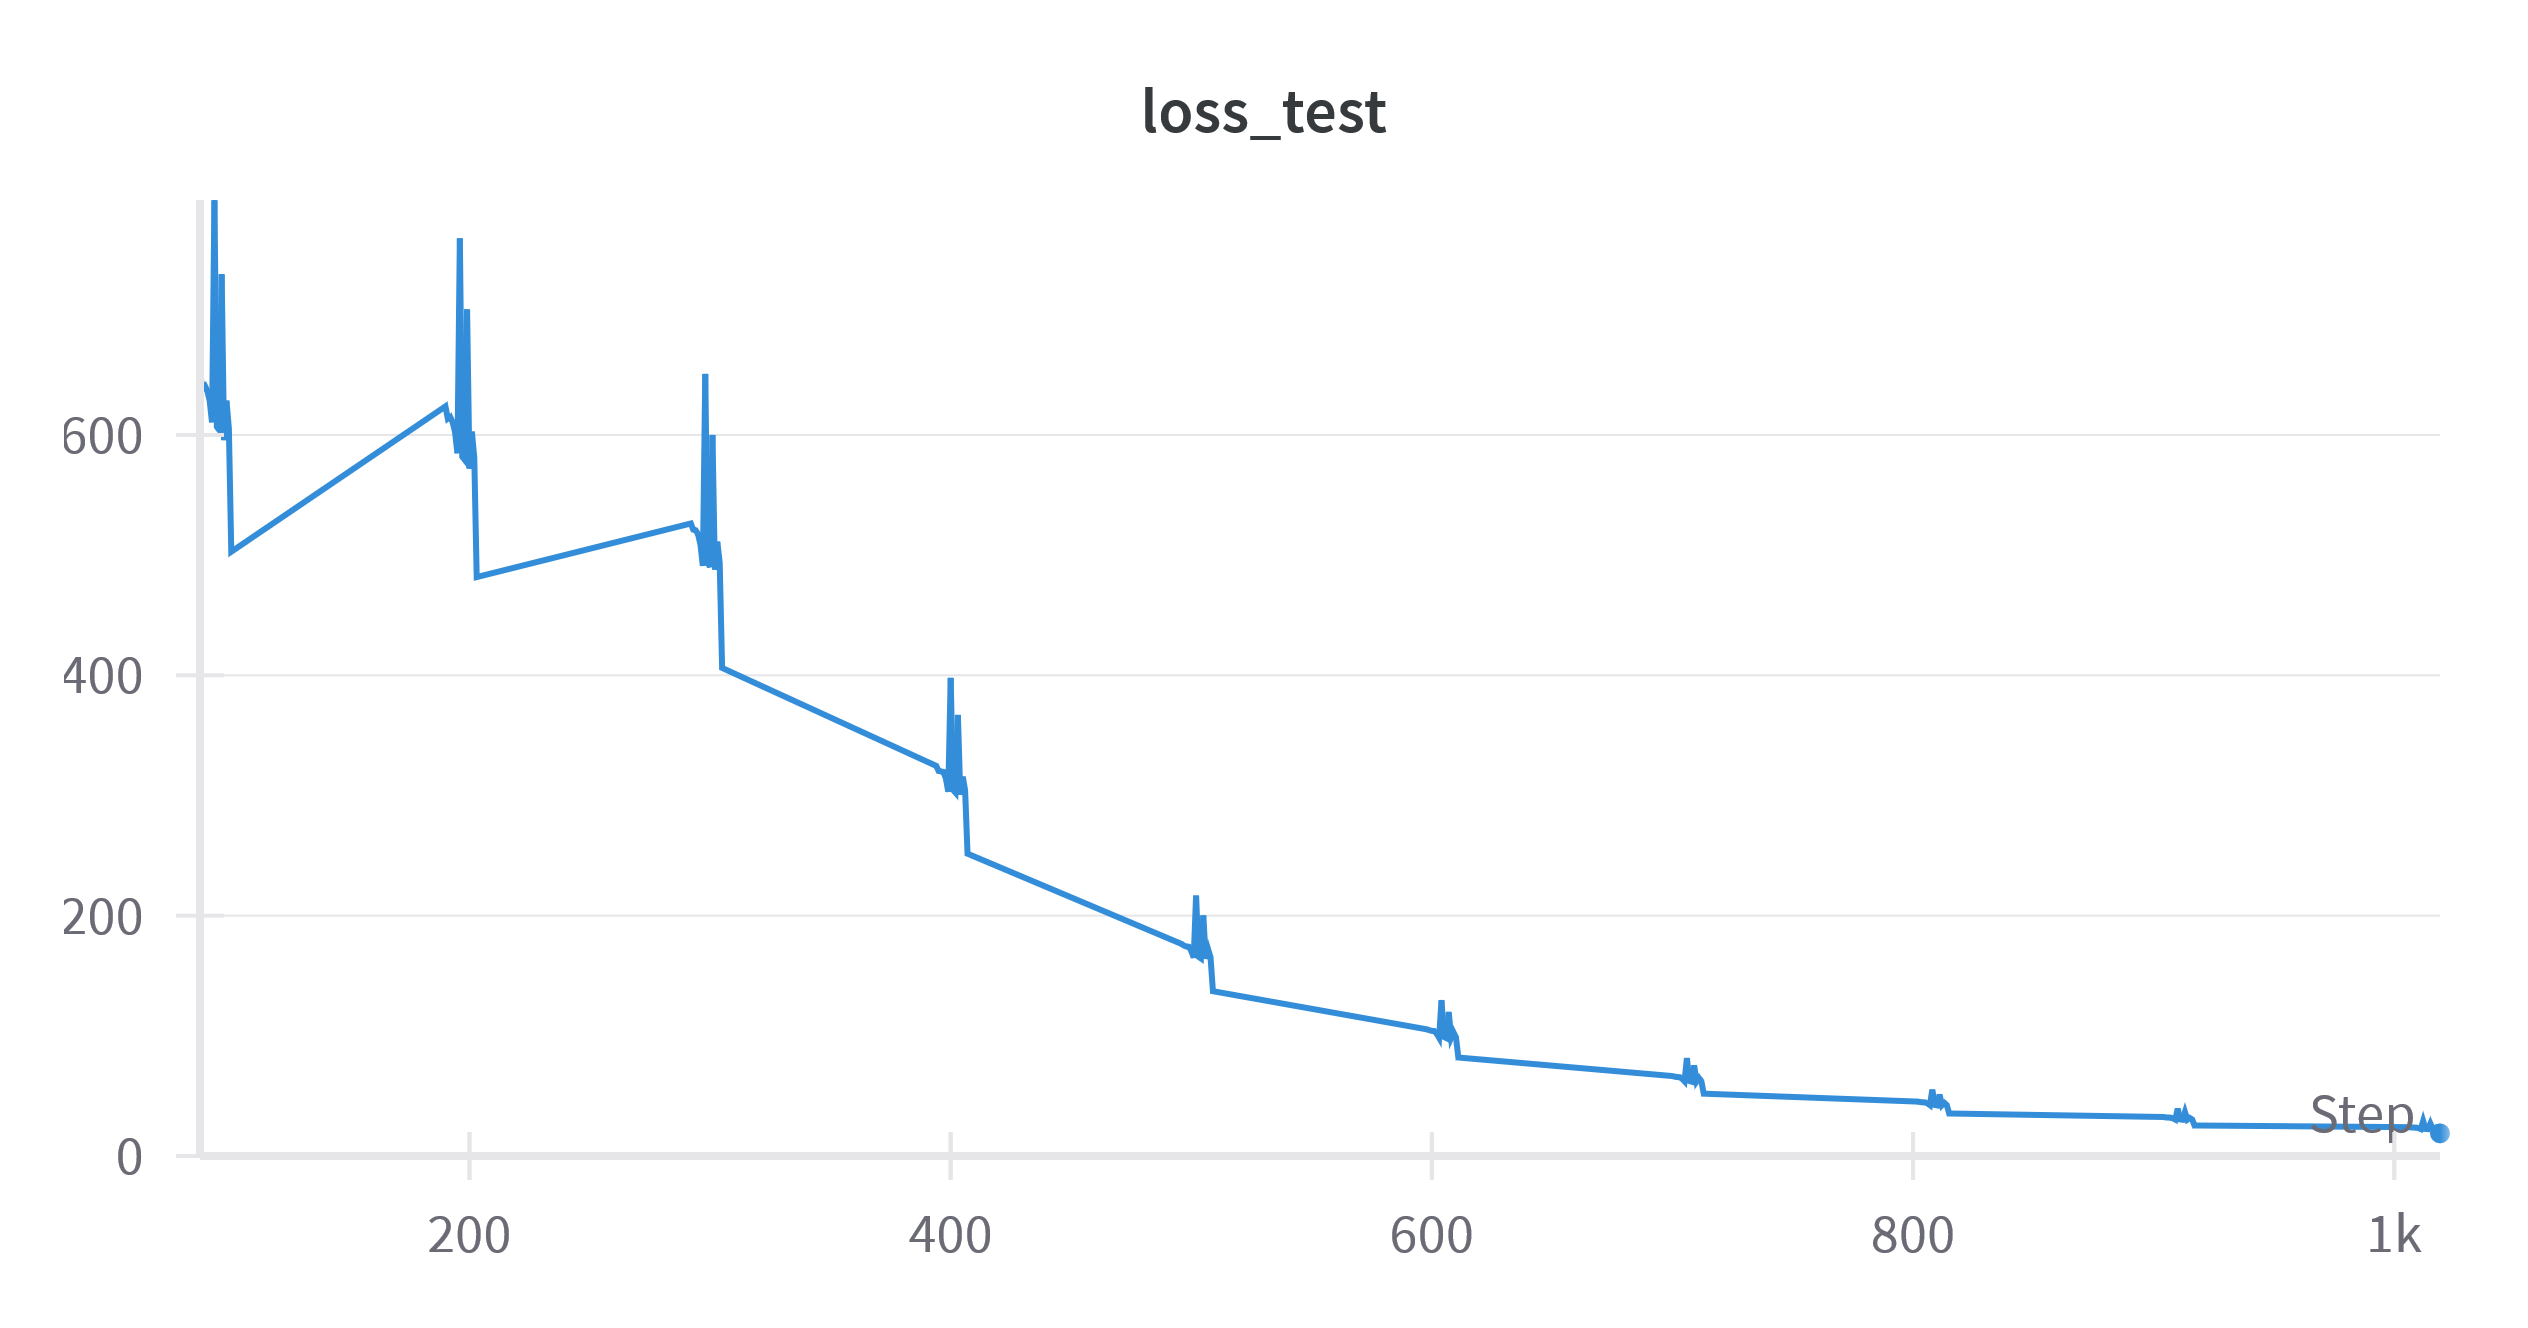
\includegraphics[width=0.45\linewidth]{figures/Figure29.png}}
    \caption{(a) Train loss (b) Test loss
    \textcolor{green}{tb adaugate info despre model si datele pe care s-au obtinut aceste rezultate}
    }
    \label{fig:fig25}
\end{figure}

\begin{figure}[!ht]
    \subfigure[]{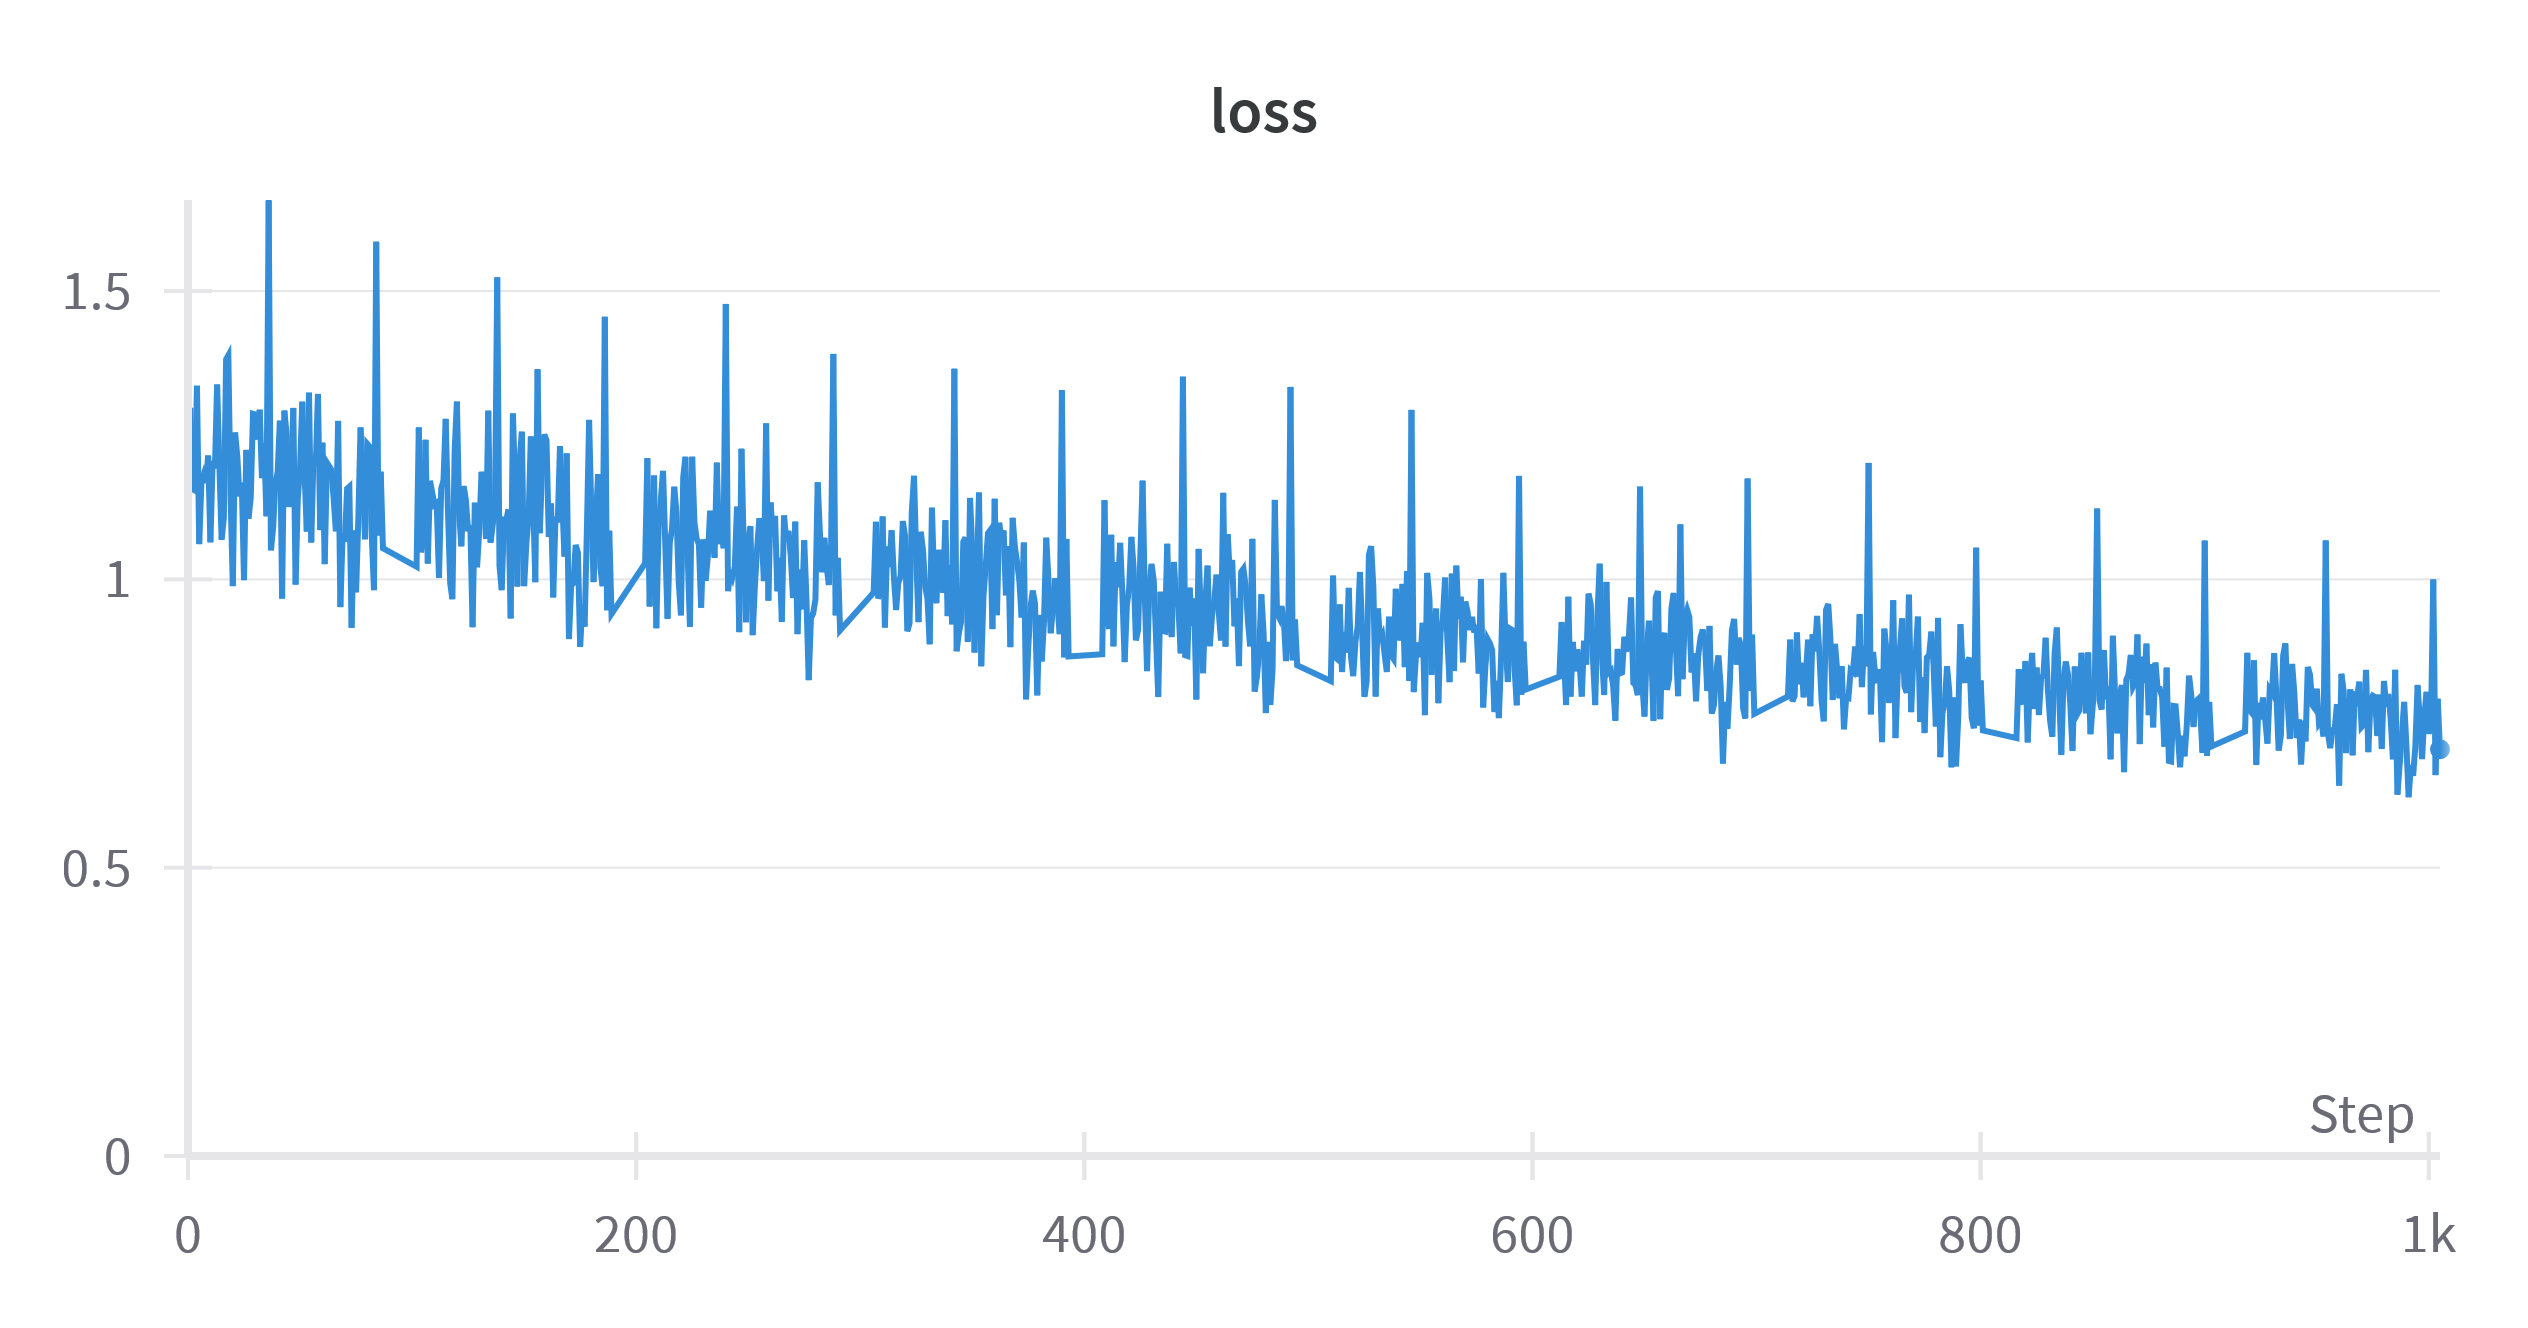
\includegraphics[width=0.45\linewidth]{figures/Figure30.png}}
    \subfigure[]{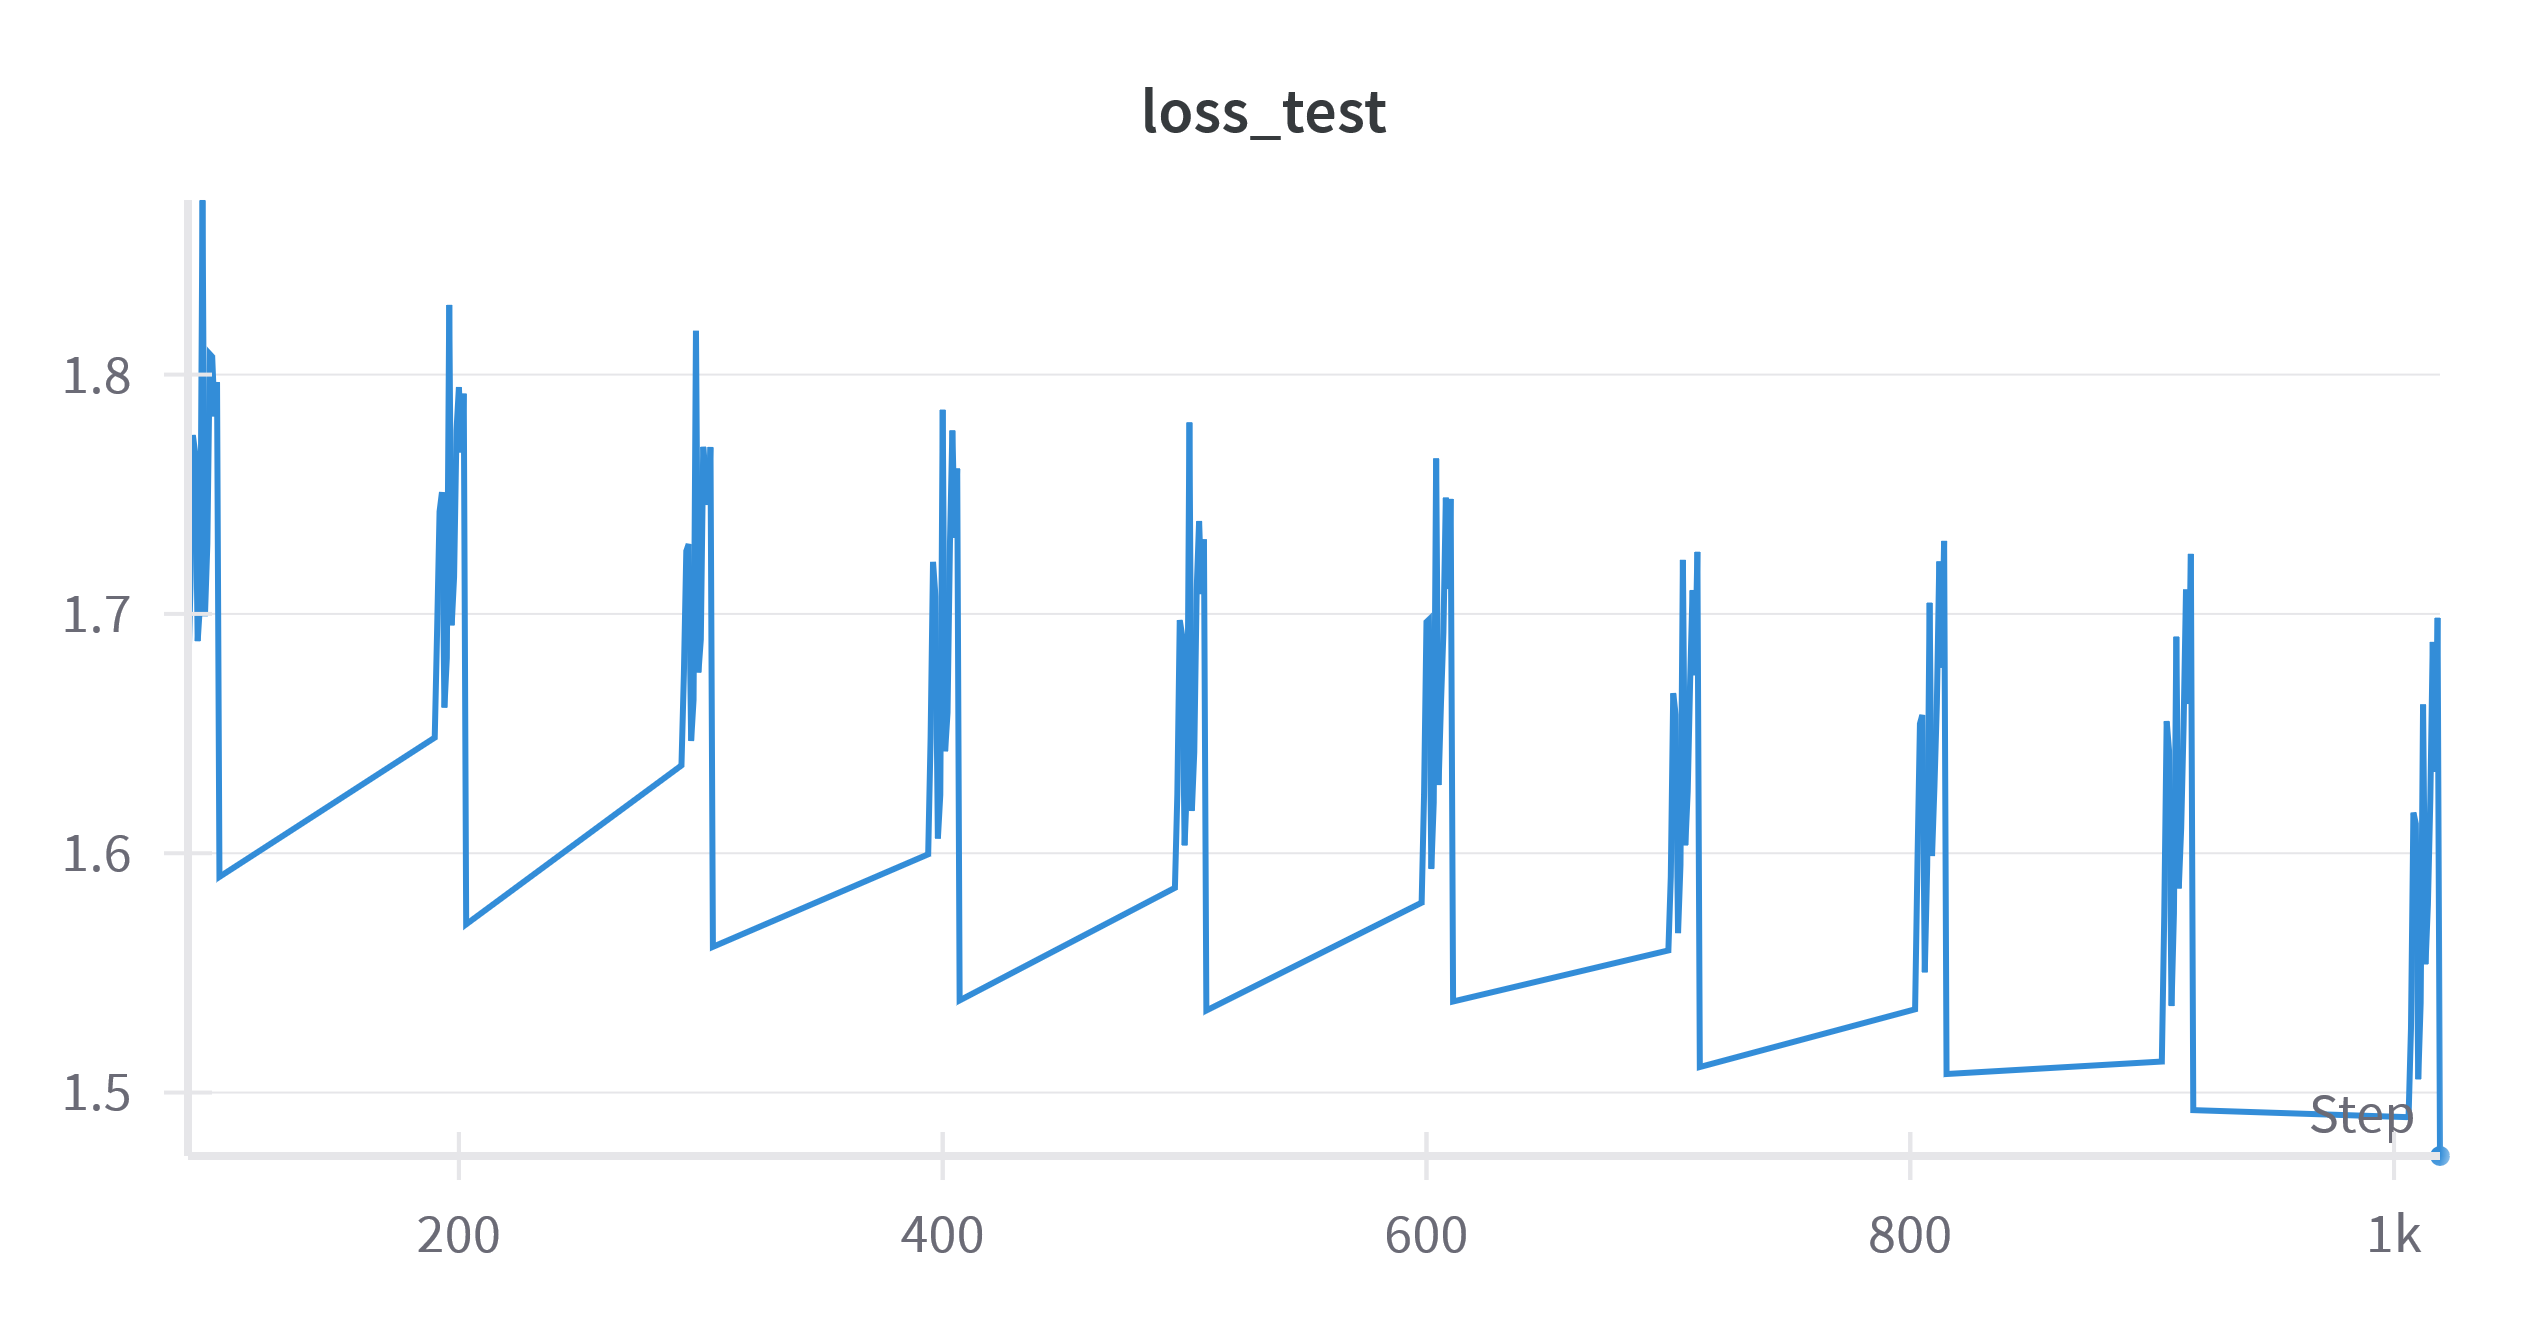
\includegraphics[width=0.45\linewidth]{figures/Figure31.png}}
    \caption{(a) Train loss (b) Test loss
    \textcolor{green}{tb adaugate info despre model si datele pe care s-au obtinut aceste rezultate}
    }
    \label{fig:fig26}
\end{figure}

\subsection{Experiment 3}

For the next experiment, I normalized the images again 
\textcolor{green}{te rog precizeaza dimensiunea} 
to see if I could get a starting loss lower than the previous ones. I also found another file containing pre-trained weights, this time from the official Effdet library on GitHub ~\cite{link7}. With this configuration, I trained 13 epochs. 
\textcolor{green}{doar head-ul sau tot modelul?}  
\textcolor{green}{tb adaugate info despre setup-ul de antrenare a head-ului / modelului (learning rate, decay, optimizator, batch size, loss, no of epochs)}

Figure \ref{fig:fig27} shows how the train and test loss looked after those 13 epochs. 
While the initial loss was much lower than the previous ones, I was not satisfied with the test loss, so I continued to experiment.

\begin{figure}[!ht]
    \subfigure[]{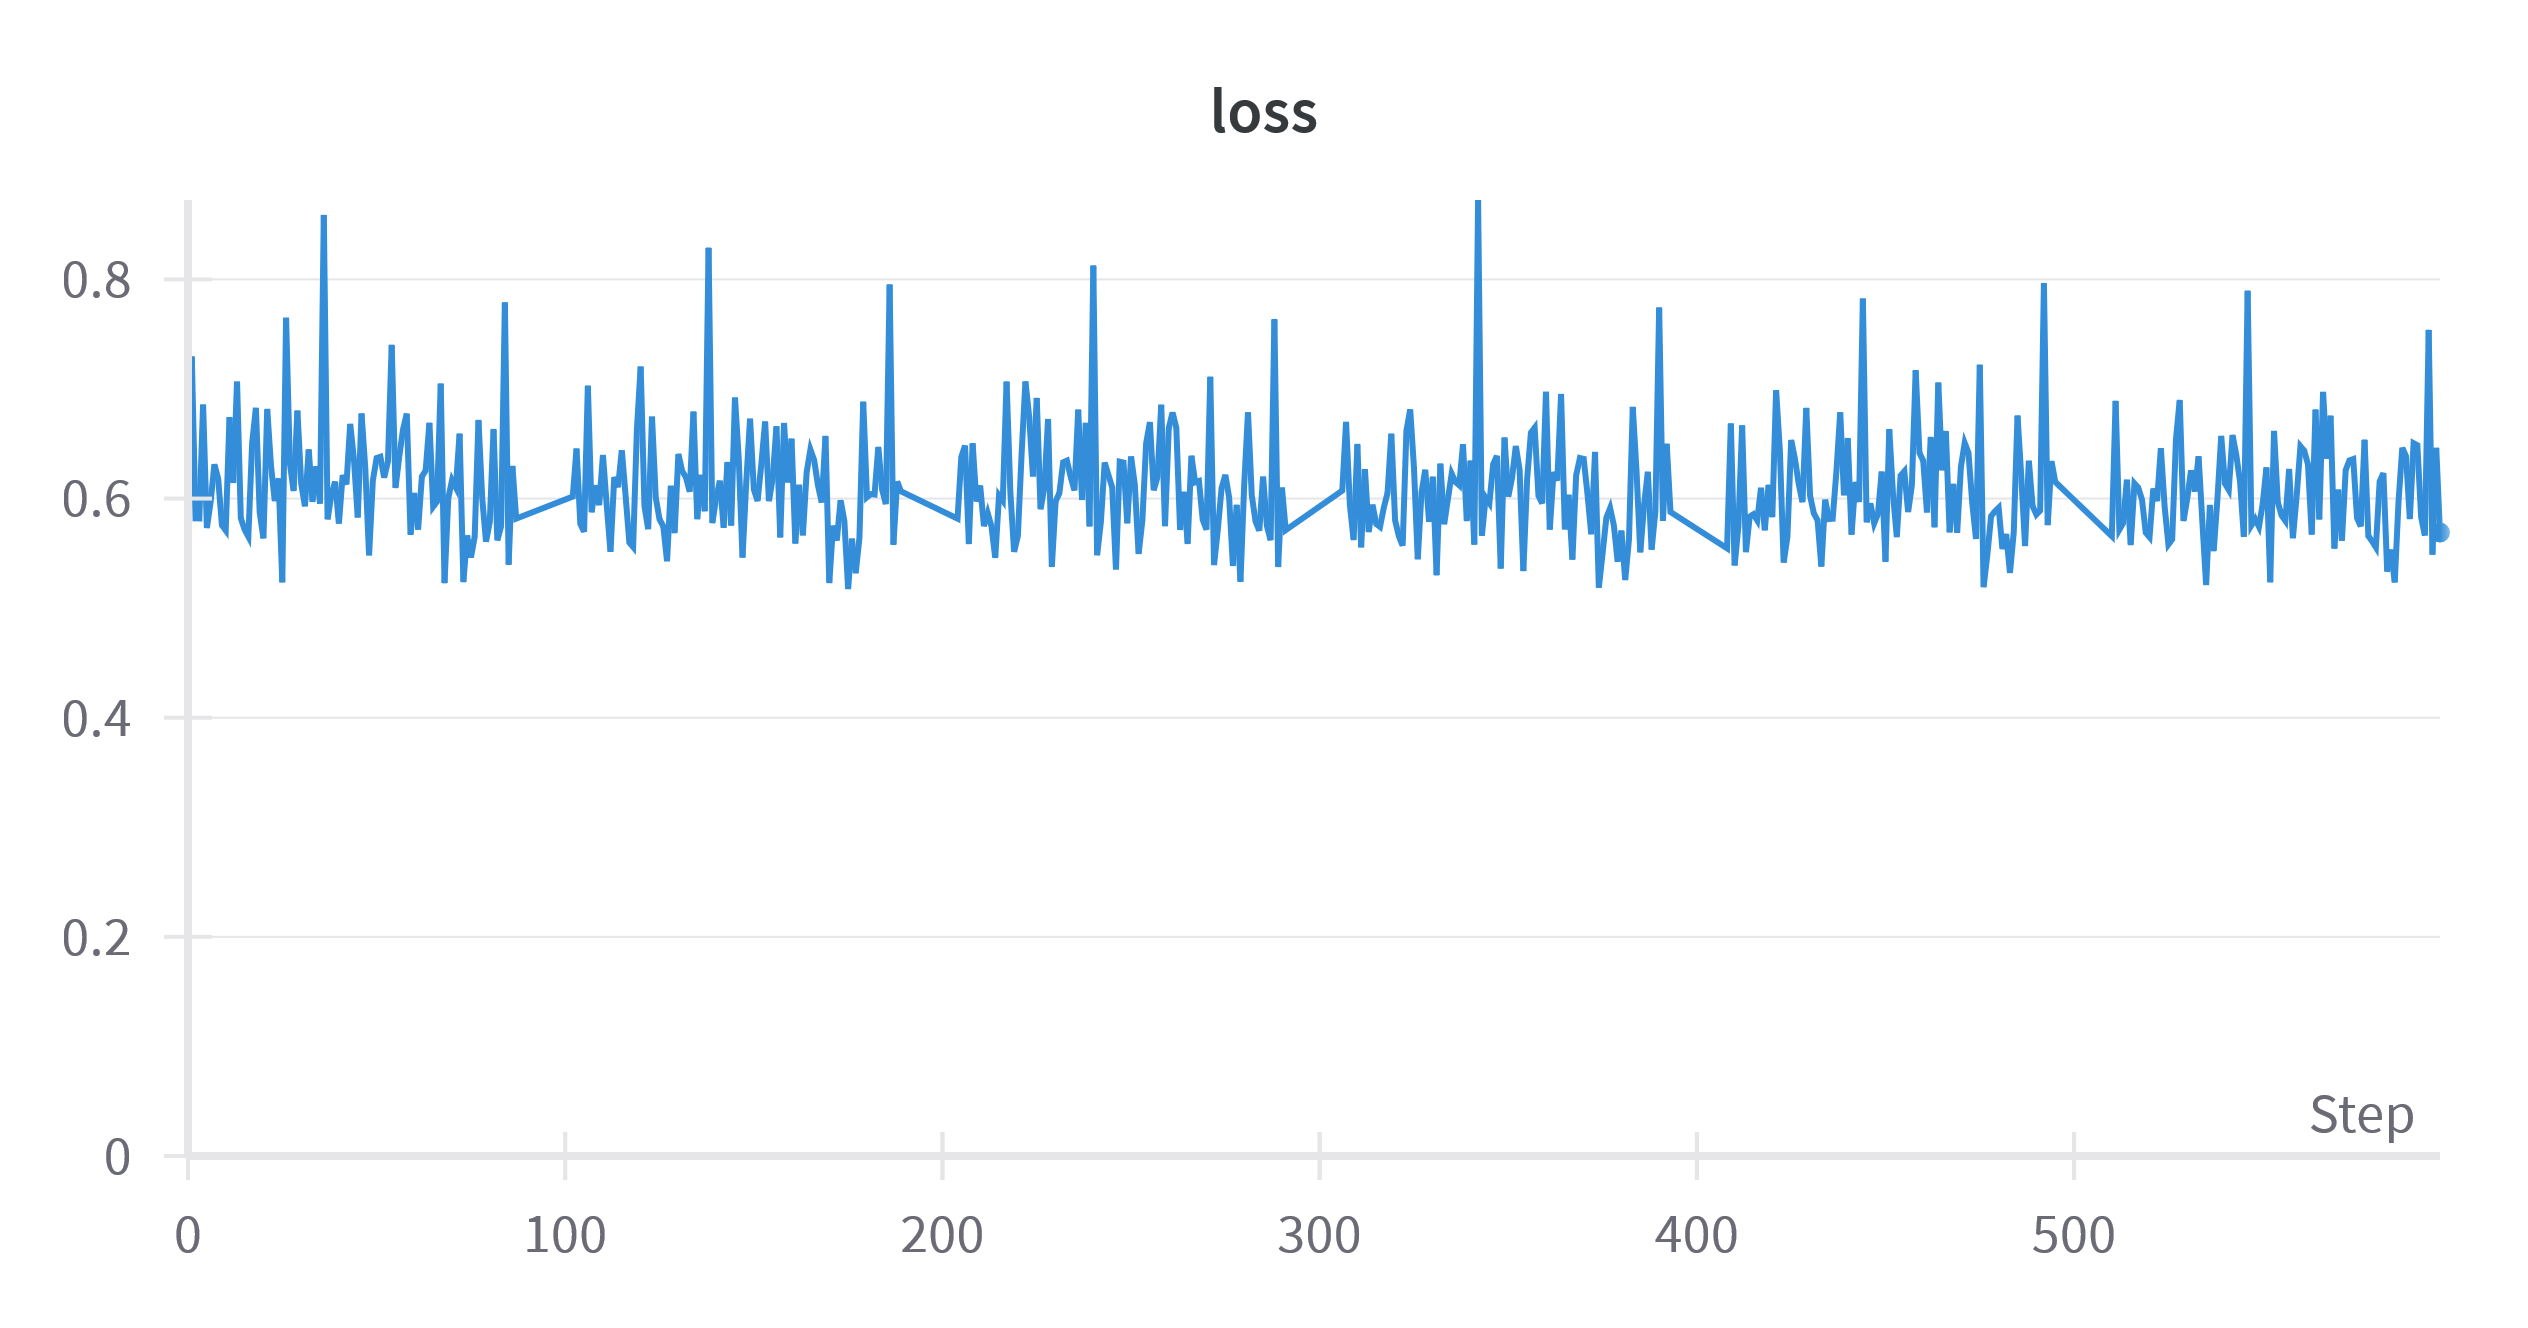
\includegraphics[width=0.45\linewidth]{figures/Figure32.png}}
    \subfigure[]{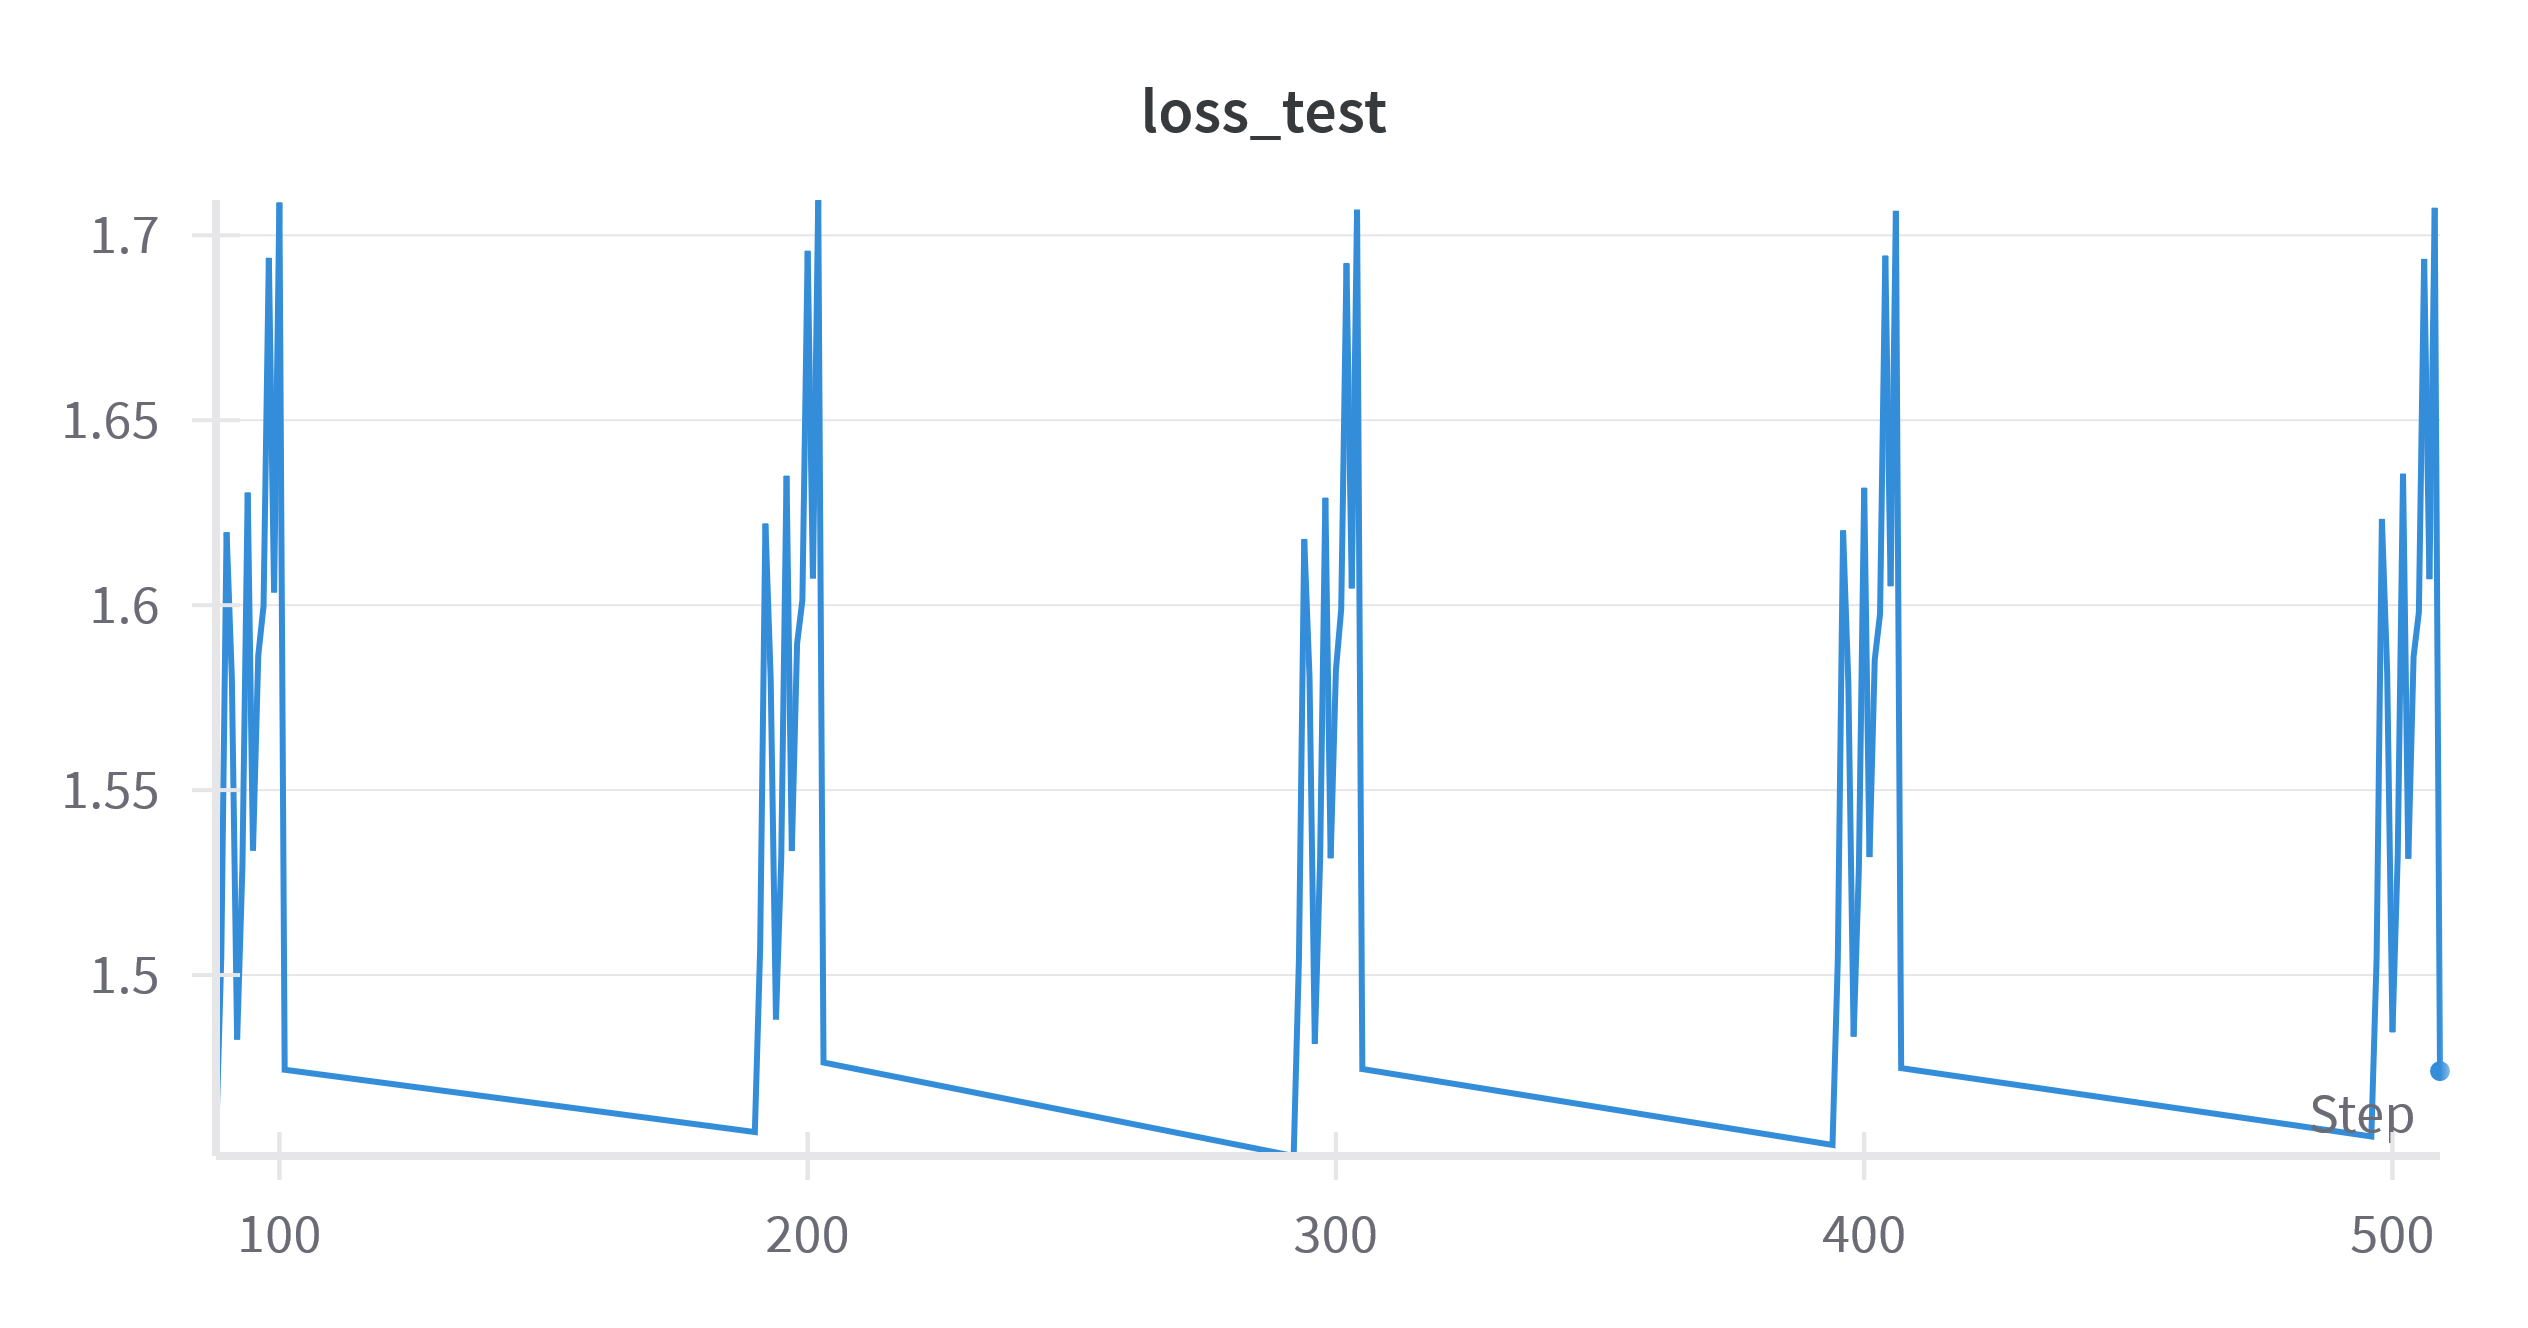
\includegraphics[width=0.45\linewidth]{figures/Figure33.png}}
    \label{fig:fig27}
    \caption{(a) Train loss (b) Test loss
    \textcolor{green}{tb adaugate info despre model si datele pe care s-au obtinut aceste rezultate}
    }
\end{figure}

\subsection{Experiment 4}

In the next experiment, I changed the learning rate decay from ReduceLROnPlateau to CosineAnnealingLR, with a minimum learning rate of \(1e^{-6}\). I also modified the way the decay is applied, calling it after the train loss rather than the test. Additionally, I modified the way the model is initialized; instead of manually downloading the file and loading a Pytorh script, I used the create\_model\_from\_config method from the Effdet library, calling it this way: \(create\_model\_from\_config(bench\_task='train', num\_classes=2, pretrained=True)\).  


\begin{table}[!ht]
    \centering
    \begin{tabular}{|c|c|c|c|c|}
        \hline
        Experiment & Image size & trained/pre-trained & (hyper)params & Performance \\
        \hline\hline
        Exp1 & 512 $\times$ 512 & trained & ? & ?\\
        \hline
        Exp2 & n $\times$ m & pre-trained & ? & ?\\
        \hline
        Exp3 & n $\times$ m & pre-trained & ? & ?\\
        \hline
        ? & ? & ? & ? & ?\\
        \hline    
    \end{tabular}
    \caption{Detection models}
    \label{tab:detectionModels}
\end{table}